%%%%%%%%%%%%%%%%%%%%%%%%%%%%%%%%%%%%%%%%%%%%%%%%%%%%%%%%%%%%%%%%%%%%%%%%%%%%%%%%
% setup.tex
% Main tex file for setup and content collocation
% For the use of University of Amsterdam
% Information Systems and Data Science students
% Adapted by Riccardo Fiorista (riccardo.fiorista@proton.me)
%%%%%%%%%%%%%%%%%%%%%%%%%%%%%%%%%%%%%%%%%%%%%%%%%%%%%%%%%%%%%%%%%%%%%%%%%%%%%%%%

% Options:
% Choose one of:
%% `is` - Information Systems
%% `ds` - Data Science 
% Add (separated by `,`):
%% `nolinenumbering` - If you want to remove line numbering on submission
%% `draftmargins` - If you would like to give your reviewer more space for comments
%% `nofrontpicture` - If you do not wish to have a graphic on your front-page
%% `nofirstcompanypicture` - If you do not wish to have a graphic on your front-page
%% `nosecondcompanypicture` - If you do not wish to have a graphic on your front-page
\documentclass[ds,nofirstcompanypicture,nolinenumbering]{mscthesis}

%%%%%%%%%%%%%%%%%%%%%%%%%%%%%%%%%%%%%%%%%%%%%%%%%%%%%%%%%%%%%%%%%%%%%%%%%%%%%%%%
% DOCUMENT METADATA
%%%%%%%%%%%%%%%%%%%%%%%%%%%%%%%%%%%%%%%%%%%%%%%%%%%%%%%%%%%%%%%%%%%%%%%%%%%%%%%%

% Thesis related entries
\title{Simulation-based inference of gravitational waves}
\subtitle{Assessing performance with state-of-the-art deep-learning models}

% Date on which your thesis is submitted
\date{30.06.2024}

% 4-5 keywords should do the trick. They should ideally be phrases of 2-4 words or single words.
\keywords{Simulation-Based Inference, Bayesian Inference, Gravitational Waves, UNet, Attention UNet, Vision Transformer, Time Series data}

% Author data
\authorname{Nicola Asquith}
\authorid{15058050}
\authoremail{nicola.asquith@student.uva.nl}

% Supervisors
\uvasupervisorname{Associate Professor, Christoph Weniger}
\uvasupervisoraffiliation{GRAPPA Institute for Theoretical Physics}
\uvasupervisoremail{C.Weniger@uva.nl}

% Comment if you do not have an external supervisor
% \externalsupervisorname{External Supervisor} \externalsupervisoraffiliation{External Supervisor}
% \externalsupervisoremail{supervisor@company.nl}

% % Uncomment and fill paths if you want to add custom images
% %% Figure size suggestions (in general it's best to render them from SVGs):
% %% 3000x3000 @ 240dpi for all three
% \titlepicturepath{}
% \firstcompanypicturepath{}
% \secondcompanypicture{path}
\usepackage{csquotes}
\usepackage{placeins}
\usepackage{afterpage}
\usepackage{adjustbox}

%%%%%%%%%%%%%%%%%%%%%%%%%%%%%%%%%%%%%%%%%%%%%%%%%%%%%%%%%%%%%%%%%%%%%%%%%%%%%%%%
% tikz library
%%%%%%%%%%%%%%%%%%%%%%%%%%%%%%%%%%%%%%%%%%%%%%%%%%%%%%%%%%%%%%%%%%%%%%%%%%%%%%%%
\usepackage{tikz}
\usetikzlibrary{shapes.geometric, arrows}

% Peregrine method

\tikzstyle{sample} = [rectangle, rounded corners, minimum width=1cm, minimum height=1cm, text centered, text width=4cm, draw=black, fill=red!30]
\tikzstyle{simulator} = [rectangle, rounded corners, minimum width=1cm, minimum height=1cm, text centered, text width=4cm, draw=black, fill=blue!30]
\tikzstyle{network} = [rectangle, rounded corners, minimum width=1cm, minimum height=1cm, text centered, text width=5cm, draw=black, fill=green!30]
\tikzstyle{inference} = [rectangle, rounded corners, minimum width=1cm, minimum height=1cm, text centered, text width=2cm, draw=black, fill=yellow!40]
\tikzstyle{pinput} = [rectangle, minimum width=1cm, minimum height=1cm, text centered, draw=black, text width=2cm, fill=pink!30]
\tikzstyle{tinput} = [rectangle, minimum width=1cm, minimum height=1cm, text centered, text width=2cm, draw=black, fill=pink!30]
\tikzstyle{output} = [rectangle, minimum width=1cm, minimum height=1cm, text centered, draw=black, fill=orange!30]

\tikzstyle{arrow} = [thick, ->, >=stealth]

% UNet architecture

\tikzstyle{input} = [rectangle, minimum width=1cm, minimum height=0.1cm, text centered, draw=white, fill=white!30]
\tikzstyle{conv} = [rectangle, minimum width=1cm, minimum height=0.1cm, text centered, draw=black, fill=orange!30]
\tikzstyle{convx2} = [rectangle, minimum width=1cm, minimum height=0.1cm, text centered, draw=black, fill=orange!30]
\tikzstyle{pool} = [rectangle, minimum width=1cm, minimum height=0.1cm, text centered, draw=black, fill=blue!30]
\tikzstyle{upconv} = [rectangle, minimum width=1cm, minimum height=0.1cm, text centered, draw=black, fill=green!30]
\tikzstyle{concat} = [rectangle, dotted, minimum width=1cm, minimum height=0.1cm, text centered, draw=black, fill=white!30]
\tikzstyle{outconv} = [rectangle, minimum width=1cm, minimum height=0.1cm, text centered, draw=black, fill=orange!30]
\tikzstyle{flatten} = [rectangle, minimum width=1cm, minimum height=0.1cm, text centered, draw=black, fill=lime!30]
\tikzstyle{fc} = [rectangle, minimum width=1cm, minimum height=0.1cm, text centered, draw=black, fill=red!30]
\tikzstyle{summary} = [ellipse, minimum width=1cm, minimum height=0.1cm, text centered, text width=1.5cm, draw=black, fill=teal!30]
\tikzstyle{AG} = [circle, dashed, minimum width=0.1cm, minimum height=0.1cm, text centered, draw=black, fill=violet!30]

\tikzstyle{arrow_unet} = [thin, ->, >=stealth]
\tikzstyle{arrow_unet_dotted} = [dashed, thin, ->, >=stealth]

% Peregrine architecture

\tikzstyle{per_input} = [rectangle, minimum width=1cm, minimum height=0.1cm, text centered, draw=black, fill=blue!30]
\tikzstyle{per_unet} = [rectangle, minimum width=1cm, minimum height=0.1cm, text centered, draw=black, fill=red!30]
\tikzstyle{per_features} = [rectangle, minimum width=1cm, minimum height=0.1cm, text centered, draw=black, fill=green!30]
\tikzstyle{per_concat} = [rectangle, dotted, minimum width=1cm, minimum height=0.1cm, text centered, draw=black, fill=white!30]
\tikzstyle{per_MLP} = [rectangle, minimum width=1cm, minimum height=0.1cm, text centered, draw=black, fill=orange!30]
\tikzstyle{per_labels} = [rectangle, minimum width=1cm, minimum height=0.1cm, text centered, draw=black, fill=cyan!30]
\tikzstyle{per_logratios} = [rectangle, minimum width=1cm, minimum height=0.1cm, text centered, draw=black, fill=magenta!30]

% Attention gate

\tikzstyle{wg} = [rectangle, text centered, draw=black, fill=blue!30]
\tikzstyle{wx} = [rectangle, text centered, draw=black, fill=blue!30]
\tikzstyle{plus} = [circle, text centered,  text width=0.2cm, draw=black, fill=white!30]
\tikzstyle{relu} = [rectangle, text centered, draw=black, fill=white!30]
\tikzstyle{psi} = [rectangle, text centered, draw=black, fill=blue!30]
\tikzstyle{sigmoid} = [rectangle, text centered, draw=black, fill=white!30]
\tikzstyle{times} = [circle, text centered, text width=0.2cm, draw=black, fill=white!30]

%%%%%%%%%%%%%%%%%%%%%%%%%%%%%%%%%%%%%%%%%%%%%%%%%%%%%%%%%%%%%%%%%%%%%%%%%%%%%%%%
% CONTENT
%%%%%%%%%%%%%%%%%%%%%%%%%%%%%%%%%%%%%%%%%%%%%%%%%%%%%%%%%%%%%%%%%%%%%%%%%%%%%%%%

\begin{document}
\pagestyle{plain}

\maketitlepage
\fixemptypage
\setcounter{page}{1}

\begin{abstract}
% A summary of results should be included. Avoid citations. Maximum length is 200 words.

The detection and analysis of gravitational waves (GW) is providing the opportunity to study the universe from a new perspective. Current methods of parameter inference from GW are computationally expensive, and the expected increase in detected events in the future is introducing significant data analytics challenges for the GW community. In this work, we focus on a specific analysis pipeline, \texttt{Peregrine}, which performs multiple sequential rounds of simulation-based inference employing the U-Net CNN architecture. The major bottleneck for performance in this pipeline is the network training time. Attention mechanisms, particularly as applied in in transformer models have become very popular in recent years due to their reported high performance. We compare the performance of \texttt{Peregrine} with the baseline U-Net model with several variations, including Attention U-Net, pre-trained Vision Transformer, pre-trained multi-variate time series transformer, and finally, structured network pruning of the original U-Net. In conclusion, we found that the best performing model was the original U-Net, and that the use of larger transformer models did not provide any performance improvement. This was predominantly due to longer training times required. The pruned networks could be trained faster but suffered from poorer accuracy in later inference rounds.
\todo[inline]{Change abstract to be consistent with latest results}

\end{abstract}

\maketitle

\section*{Github Repository}
\url{https://github.com/Nic0laA/master-thesis}

% Sections; Try to stick to this setup but you can comment each section
\section{Introduction}
\label{sec:introduction}
% Mention scientific context/field, problem statement, research gap and candidate (sub) research question(s). 
\stepcounter{footnote}
\footnotetext{Cover image: Chat GPT-4o}

Gravitational Waves (GW) are ripples in the fabric of space-time originating from the acceleration of massive astronomical objects e.g. the merger of black holes or neutron stars. The study of gravitational waves is allowing us to observe the universe in an entirely new way.

Since the first direct detection of gravitational waves in 2015~\cite{LIGO_2016}, the detector sensitivities and survey volumes are ever-increasing. The continuous rise in detection of events over time is introducing significant data analysis challenges for the gravitational wave community~\cite{bhardwaj2023peregrine}.
For instance, current data analysis pipelines are not equipped to deal with independent signals arriving coincidentally in detectors, and scale poorly as the dimensionality of the problem increases~\cite{alvey2023things}. This makes the analysis of large number of overlapping signals, or those containing non-stationary noise increasingly complicated and computationally very expensive~\cite{bhardwaj2023peregrine}.

The \texttt{peregrine} inference pipeline has been developed at the UvA GRAPPA institute to help address some of these challenges~\cite{bhardwaj2023peregrine}. It utilises the Simulation-based inference (SBI) method based on the TMNRE (Truncated Marginal Neural Ratio Estimation) algorithm with the U-Net Convolutional Neural Network (CNN) architecture. The \texttt{peregrine} pipeline incorporates multiple rounds of sequential network training and inference, which comes with a high computation cost. Since the main bottleneck is currently the training time of the network ($\sim$80\% of total runtime), it would be highly beneficial for the network underlying \texttt{peregrine}~\cite{bhardwaj2023peregrine} to be as fast and as accurate as possible. This study explores the possibilities to improve the \texttt{peregrine} pipeline using state-of-the-art neural network architectures.

In the study, we compare the original U-Net model with two pre-trained transformer models~\cite{Dosovitskiy_2021_ViT,Zerveas_2020_mvts}, Attention U-Net~\cite{Oktay_2018_AUNet}, as well as use pruning methods~\cite{Fang_Ma_Song_Mi_Wang_2023} to reduce the number of trainable parameters in the current U-Net model. It is important to note that the information \texttt{peregrine} can extract from the GW signal is already at the statistical limit due to measurement noise in the signal. Therefore it is not possible to improve upon the quality of the results further, and thus the aim is rather to reach the same accuracy in a shorter period of time.

We provide background and context for the work in section~\ref{sec:related_work}, where we describe the current state of gravitational wave analysis methods and introduce the methodologies and network architectures relevant for the remainder of the work. Description of the data, the \texttt{peregrine} pipeline and how the changes to network architecture were implemented and evaluated are given in the methodology section on page~\pageref{sec:methodology}. Results and discussion are presented in sections~\ref{sec:results} and~\ref{sec:discussion} respectively. Finally, conclusions and future outlook can be found in section~\ref{sec:conclusion} on page~\pageref{sec:conclusion}.

\subsection*{Research question}

\noindent \textit{RQ: To what extent can different network architectures in \texttt{peregrine} reduce the training time, while still producing the same results as the original \texttt{peregrine}?}

\noindent \textit{SRQ1: What is a suitable metric to assess the performance of the underlying neural network (taking into account both accuracy and training time)?}

\section{Related Work}\label{sec:related_work}
% Your work needs to be grounded and compared to earlier work and the state-of-the-art. Start the section with announcing the research gap and also end with the research gap. Consider using hypotheses. 

\subsection{Gravitational Wave analysis}

The first direct detection of gravitational waves occurred in 2015 after the merger of two black holes about 1.3 billion light years away~\cite{LIGO_2016}. Since then, there have been three observing runs by the LIGO-Virgo collaboration which have yielded 90 confirmed gravitational wave detections . Of these 90 detections, 83 were binary black hole mergers, 2 were binary neutron star mergers, 3 were neutron star-black hole mergers and 2 involved the merger between a black hole and a `mystery' object that had a mass in between that of a neutron star and black hole~\cite{LIGO_FAQ_Website}. The next observing runs, O4 (started May 2023) and O5 (planned for 2027 and beyond) are predicted to detect a significant increase in events, $~\sim5\times$ more events each corresponding observing run~\cite{Petrov_2022}.

Analysis of gravitational waves is divided into two parts -- detection and parameter inference~\cite{bhardwaj2023peregrine}. In this study, we consider only the inference part, whereby given a detected waveform, we are trying to infer the physical properties of the source that generated it, as well as the distance, position and orientation in the sky relative to Earth etc.

\todo[inline]{Rewrite paragraph below}
The theory of how sources emit gravitational waves is well established, and the entire gravitational waveform may be expressed by $\sim$15 parameters~\cite{Thrane_Talbot_2019}. 
There are well established methods for accurately forward modelling GW waveforms, detector responses and instrument noise~\cite{alvey2023things} e.g.~the open-source Bilby code~\cite{Ashton_Bilby_2019,Romero_Bilby_2020,Ashton_Talbot_Bilby_2021}. Therefore, given the well-known theory, and these 15 parameters as input, it is fairly straightforward to accurately simulate what you expect the GW waveform to look like. However, performing the inverse of this problem i.e.~backing out the 15 parameters from a given GW waveform is significantly more challenging. Bayesian inference methods are therefore used extensively in gravitational-wave astronomy~\cite{Thrane_Talbot_2019}.

\todo[inline]{Rewrite paragraph below}
Due to the high dimensionality, brute-force techniques for GW parameter inference are computationally infeasible. The traditional approach involves using stochastic sampling methods~\cite{Thrane_Talbot_2019}, such as Markov chain Monte Carlo (MCMC)~\cite{Metropolis_1953,Hastings_1970} or nested sampling~\cite{Skilling_2004}. However, these techniques increasingly struggle with higher dimensional data and are not feasible options in the case of overlapping signals, where one needs to now infer 30 model parameters from the data~\cite{alvey2023things}.


\subsection{Swyft and Peregrine}



The \texttt{Peregrine} code was developed to study broad classes of gravitational wave signals. The papers describing the development of the code~\cite{bhardwaj2023peregrine,alvey2023things} will form the main starting point of this thesis, and will also serve as the baseline for this new work to be benchmarked against. \texttt{Peregrine} implements an SBI algorithm known as Truncated Marginal Neural Ratio Estimation (TMNRE)~\cite{Miller_TMNRE_2021} and is built on top of the \texttt{swyft} code~\cite{Miller2022}. The TMNRE algorithm estimates the marginal likelihood-to-evidence ratio, and works by training binary classifiers to distinguish jointly drawn sample pairs from marginally drawn sample pairs.

Summary statistics to MLP which calculates the log ratios.

\subsection{Neural Network Architectures}

\subsubsection{U-Net}

U-Net is a fully convolutional neural network that was originally developed in 2015 for biomedical image segmentation~\cite{Ronneberger_Fischer_Brox_2015}. U-Net is efficient and fast to train, and has thus become highly popular and the \enquote{gold standard} for segmenting 2D medical images for which new architectures should be benchmarked against~\cite{Sengara_2022}. The defining feature of U-Net is its symmetrical architecture consisting of a contracting path (encoder) followed by an expansive path (decoder). In the original U-Net~\cite{Ronneberger_Fischer_Brox_2015}, each step in the encoding path consists of two 3$\times$3 convolutions (unpadded in the original) doubling the number of feature channels, a ReLU and 2$\times$2 max pooling with stride 2 for downsampling. The decoding path then follows with a 2$\times$2 \enquote{up-convolution} halving the number of feature channels, concatenation with the matching feature map from the contractive path, followed by two 3$\times$3 convolutions and ReLU operations. The architecture of U-Net, reproduced from~\cite{Ronneberger_Fischer_Brox_2015}, is shown in Figure~\ref{fig:unet_arch}.

\begin{figure}
    \centering
    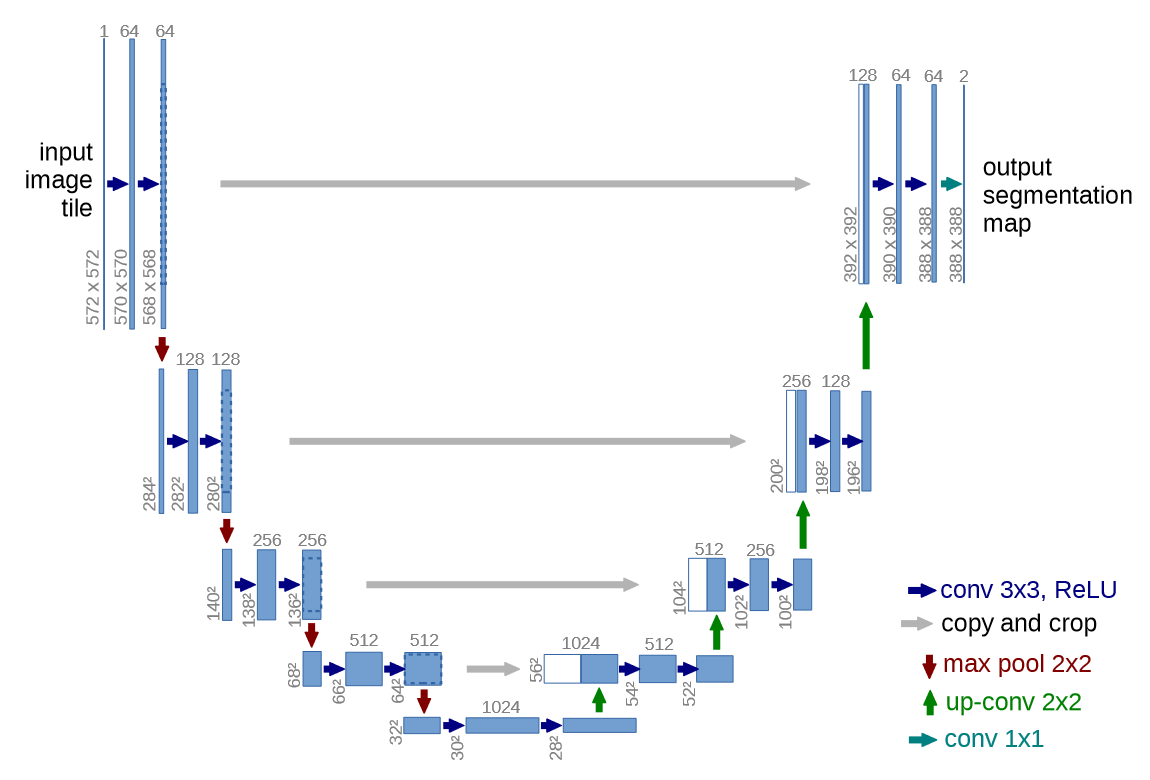
\includegraphics[width=1\linewidth]{media/images/UNet_arch.png}
    \caption{The U-Net architecture with a 2D image of resolution 572$\times$572 as example. Reproduced from~\cite{Ronneberger_Fischer_Brox_2015}.}
    \label{fig:unet_arch}
  \end{figure}

\subsubsection{Attention U-Net}

Due to the success of the U-Net architecture, several variants have since been proposed,including U-Net++~\cite{Zhou_2018_unet++} and attention U-Net~\cite{Oktay_2018_AUNet}. U-Net++
replaces the plane skip connections in vanilla U-Net with nested dense skip connections. This is to reduce the semantic gap between the encoder and decoder, which they claim yields significant performance gains.

The Attention U-Net introduces an attention gate (AG) in order to filter the features that are passed through the skip connections. The authors claim that this increases the models sensitivity and prediction accuracy with minimal impact to the computational cost. They do this by suppressing irrelevant features and learn to only focus on the most important features. 

Additive soft attention

\subsubsection{Transformer models}

Transformer models have proven widely succesful in the field of natural language progressing~\cite{Vaswani_2017_transformer} and computer vision~\cite{Dosovitskiy_2021_vit}. They provide a highly efficient platform for processing sequential data. Vision Transformers (ViT) have shown 

Vision transformers and time series models.

The use of transformer models for 1D signals is much less widespread, but~\cite{Nguyen_Miah_Bilodeau_Bouachir_2022} have shown they were very effective at extracting features from 1D signals, specifically detecting Parkinson's disease by analysing a patients gait. 

Transformers often require large amounts of training data and computing power before they are able to outperform task-specific models.

\subsection{Network pruning}

The implementation of attention U-Net and transformers models will increase the number of trainable parameters. This will likely place an additional overhead on the calculation time of \texttt{Peregrine} or require more training data. In order to reduce the number of model parameters pruning techniques exist such as \cite{Fang_Ma_Song_Mi_Wang_2023}.


%\section{Background Theory}
\label{sec:background_theory}

\subsection{Simulation-based inference}
\label{sec:background_theory_sbi}





\section{Methodology}
\label{sec:methodology}
% Focus on what you add to the existing method. Explain what you will do and why (and how). Do not forget to characterize your research design. There should be an evaluation plan in this section. (For DS students, this normally means using manually labelled or ground truth data.)

\todo[inline]{Very much still a work in progress}

% ============================================================================ %
% Description of the data
% ============================================================================ %
\subsection{Description of the data}

The data used in this study was simulated using the open-source Bilby code~\cite{Ashton_Bilby_2019}. The gravitational waveforms of three LIGO detectors (Hanford, Washington and Livingston) were generated as a function of 15 independent parameters. Ten of these parameters represented intrinsic properties of the source e.g. the masses and spins of the two black holes, while five of these are extrinsic parameters e.g. the distance from the source and orientation in the sky with respect to the observations. Further details of the parameters are listed in Table~\ref{tab:gw_parameters}. Simulating the waveforms for training the neural network is necessary since we need $\sim$100000 waveforms for training and experimentally measured signals are rare (only 90 detections so far).

Only low SNR case considered because high SNR is unrealistic and it is important for the network to determine signal from noise.

\todo[inline]{Complete table}

\begin{table}[htb]
\centering
\begin{tabular}{|l|l|l|l|}
\hline
\textbf{Parameter} & \textbf{Type} & \textbf{Prior} & \textbf{Test Value} \\
\hline
Mass ratio, \( q \) & I & \( U(0.125, 1) \) & 0.8858 \\
Chirp mass \( M \) [\( M_{\odot} \)] & I & \( U(25, 100) \) & 32.14 \\
Inclination angle \( \theta_{jn} \) [rad] & I & sine(0, \( \pi \)) & 0.4432 \\
Phase \( \phi_c \) [rad] & I & \( U(0, 2\pi) \) & 5.089 \\
Tilt angle \( \theta_1 \) [rad] & I & sine(0, \( \pi \)) & 1.497 \\
Tilt angle \( \theta_2 \) [rad] & I & sine(0, \( \pi \)) & 1.102 \\
Spin \( a_1 \) & I & \( U(0.05, 1) \) & 0.9702 \\
Spin \( a_2 \) & I & \( U(0.05, 1) \) & 0.8118 \\
Spin angle \( \phi_{12} \) [rad] & I & \( U(0, 2\pi) \) & 6.220 \\
Spin angle \( \phi_{jl} \) [rad] & I & \( U(0, 2\pi) \) & 1.885 \\
Luminosity Distance \( d_L \) [Mpc] & E & \( U_{\text{vol}}(100, 2000) \) & 900 \\
Right ascension \( \alpha \) [rad] & E & \( U(0, 2\pi) \) & 5.556 \\
Declination \( \delta \) [rad] & E & cosine(-\( \pi/2 \), \( \pi/2 \)) & 0.071 \\
Polarisation angle \( \psi \) [rad] & E & \( U(0, \pi) \) & 1.100 \\
Merger time \( t_c \) [GPS s] & E & \( U(-0.1, 0.1) \) & 0.000 \\
\hline
\end{tabular}
\caption{Description and type of the parameters that fully describe the detected gravitational waves.}
\label{tab:gw_parameters}
\end{table}

The waveform data consists of 1D signals in both time and frequency domains, collected from the three separate detectors that have captured the event simultaneously. An example of the signal in the time domain is shown in Figure~\ref{fig:obs_time_domain}. In total, there are 8192 channels corresponding to 4\,s of collection time at a sampling frequency of 2048\,Hz. With the Fourier transform, the time signal is decomposed into its constituent frequency components. Both the time and frequency domains are fed into the neural network, since they have different information about the parameters encoded. An example of the signal in the frequency domain is shown in Figure~\ref{fig:obs_freq_domain}.

\begin{figure}
  \centering
  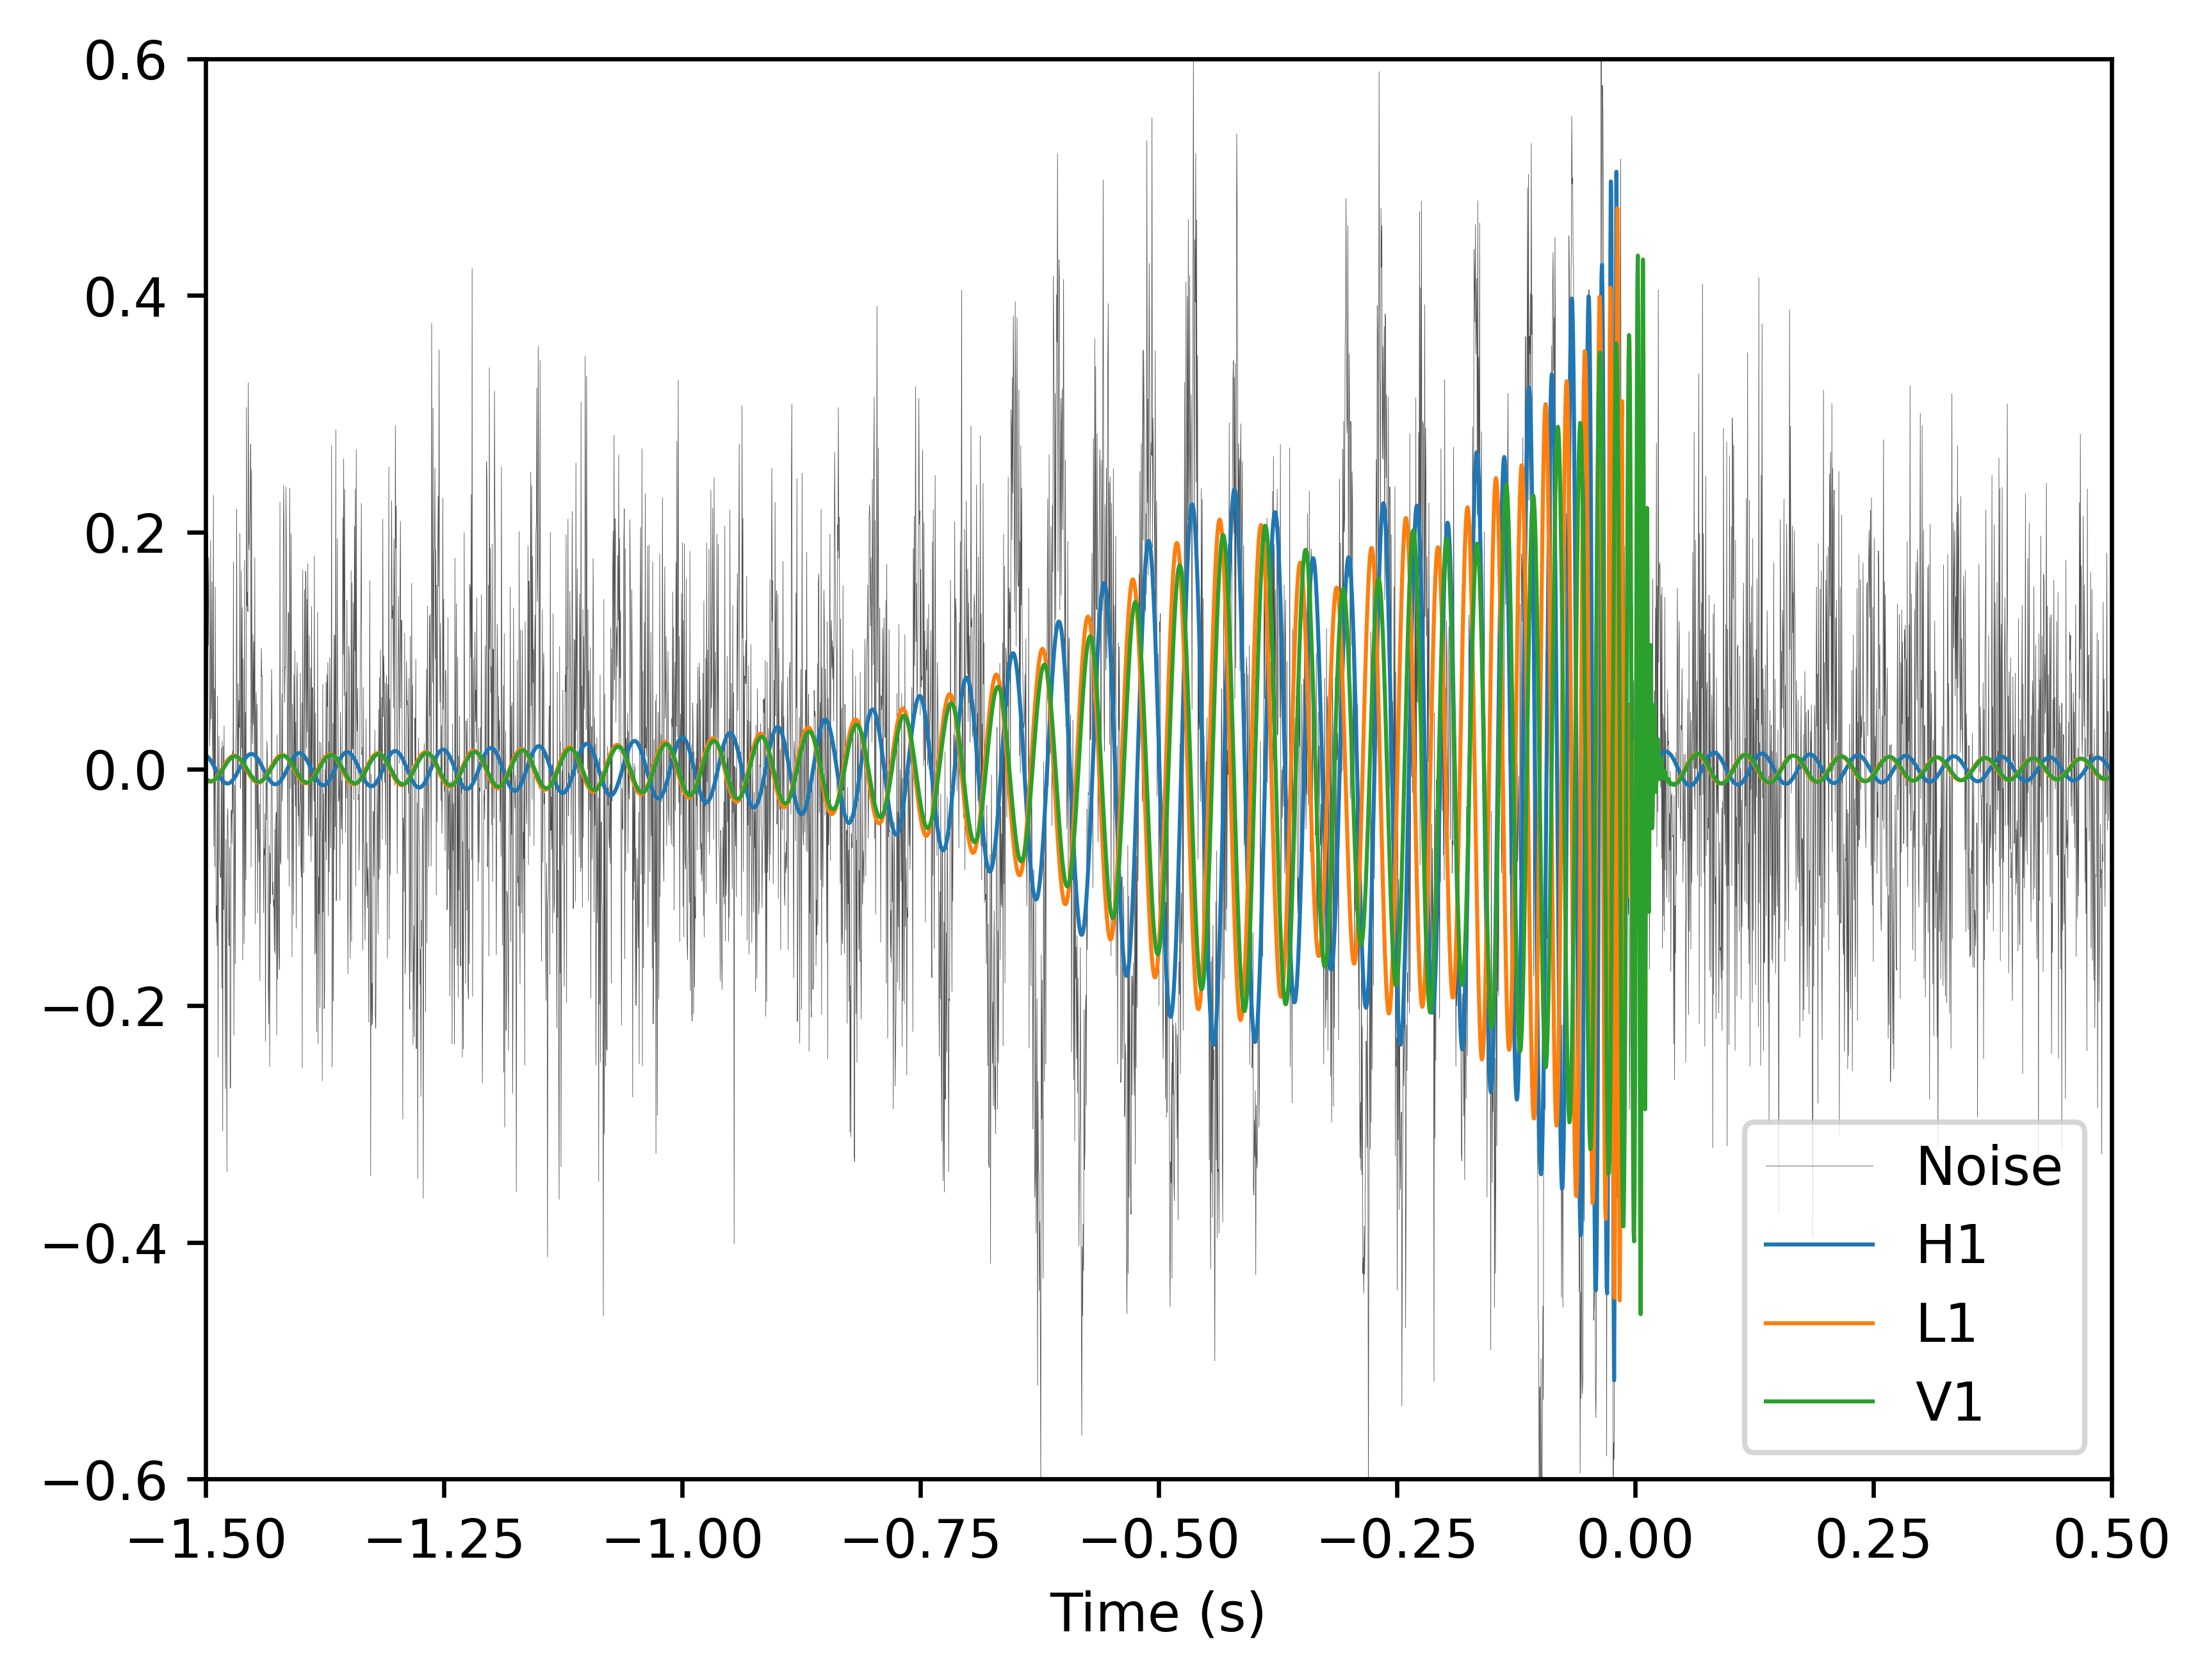
\includegraphics[width=1\linewidth]{media/images/obs_time_domain_lowSNR.png}
  \caption{Example of generated gravitational wave signal in the time domain. Signals from three detectors are shown. For clarity, the noise and signal are shown separately in the figure, but are added together when training the network. The two black holes merge at the moment t=0s. }
  \label{fig:obs_time_domain}
\end{figure}

\begin{figure}
  \centering
  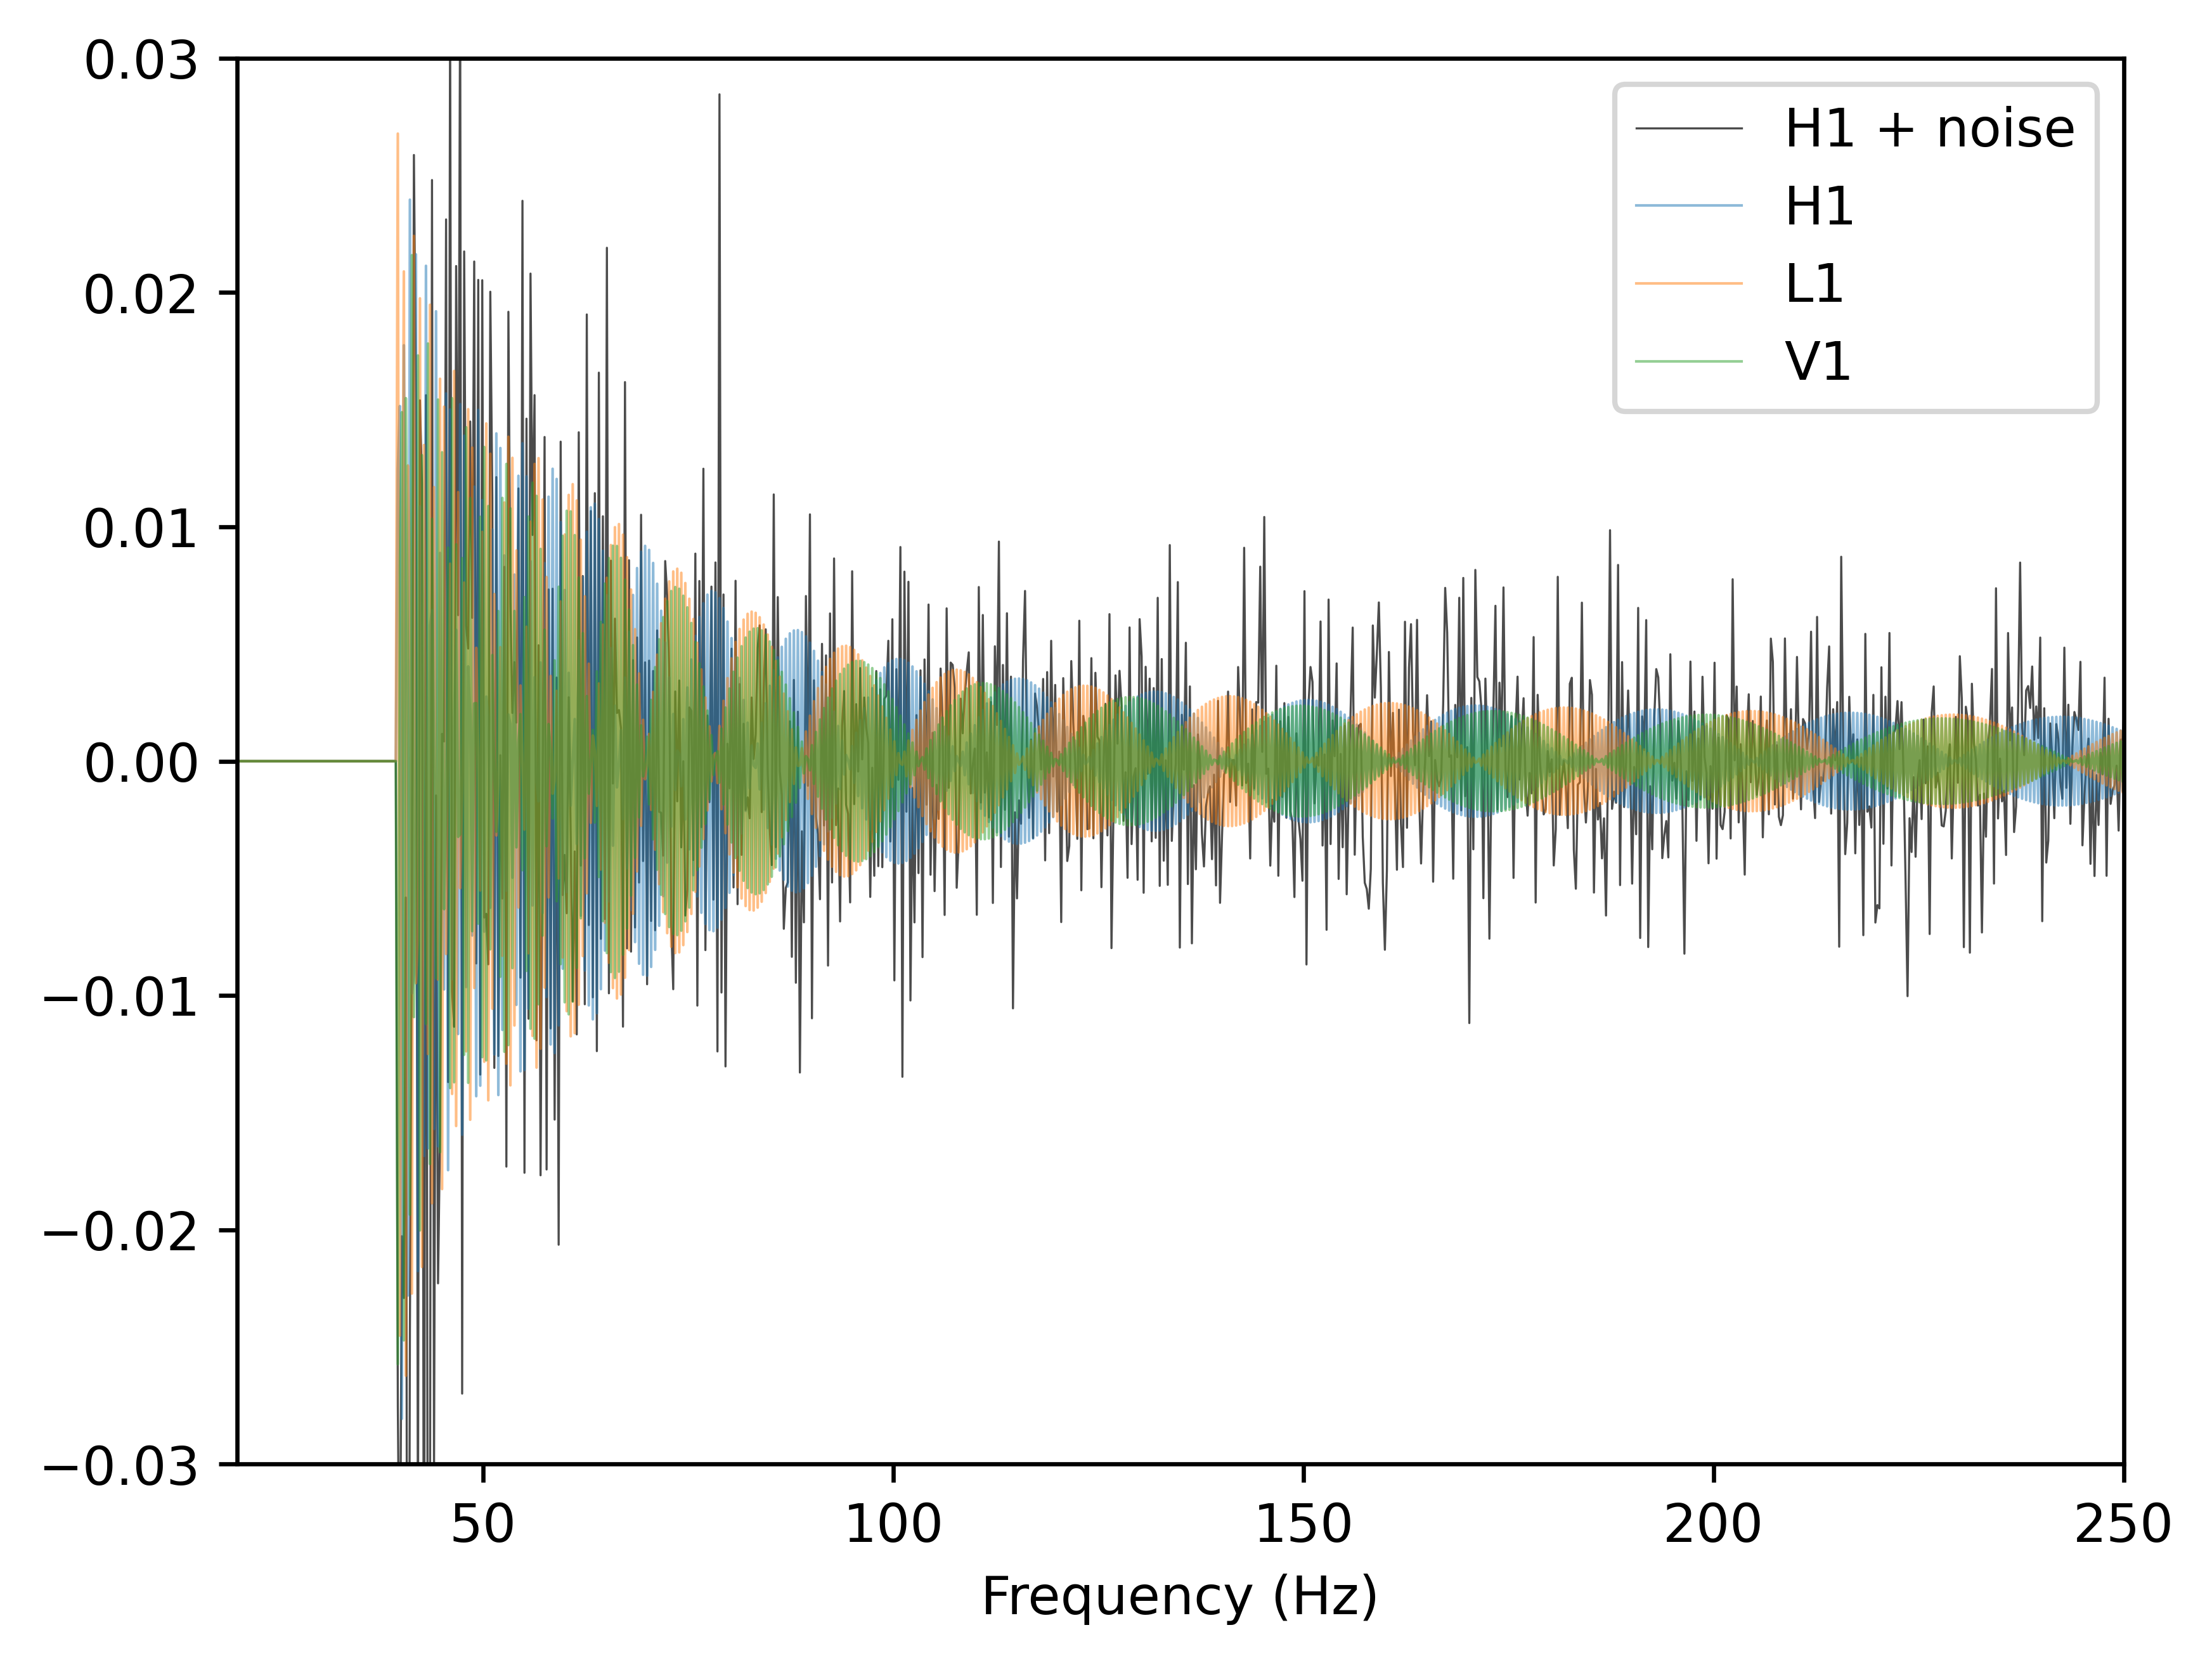
\includegraphics[width=1\linewidth]{media/images/obs_freq_domain_lowSNR.png}
  \caption{Example of generated gravitational wave signal in the frequency domain. Signals from three detectors are shown. For clarity, the noise and signal are shown separately in the figure, but are added together when training the network.}
  \label{fig:obs_freq_domain}
\end{figure}

Only low signal to noise signal will be considered here since the high SNR is unphysical and the low SNR is more challenging. Many moving parts to problem - number of truncation rounds, the number of simulations per round, network architecture, the truncation, the sampling strategy of the priors.

% ============================================================================ %
% Peregrine
% ============================================================================ %
\subsection{Peregrine inference pipeline}

The overall objective of this work is to increase the efficiency of the \texttt{Peregrine} data analysis pipeline. The work will begin with reproducing the results from papers~\cite{bhardwaj2023peregrine} and~\cite{alvey2023things}, as this will form the benchmark to which the eventual results will be compared to.

The workflow for the simulation-based inference technique for the analysis of the gravitational wave signals as implemented in \texttt{peregrine}~\cite{bhardwaj2023peregrine} is shown in Figure~\ref{fig:peregrine_pipeline}. The process starts by setting the 15 parameters of the `target observation' and then generating the example waveform to be analysed. This is done so there are `ground-truth' parameter values that you can compare your final posterior probability density distributions with and validate the overall method. If we use a true experimentally measured signal, then we can never know for certain what the `ground-truth' values of the parameters are. Given the accuracy that we can forward model the GW signals with, once the method is validated with the simulated waveforms, it is expected to work equally well with true experimental measurements.

\begin{figure}[htb]
    \centering
    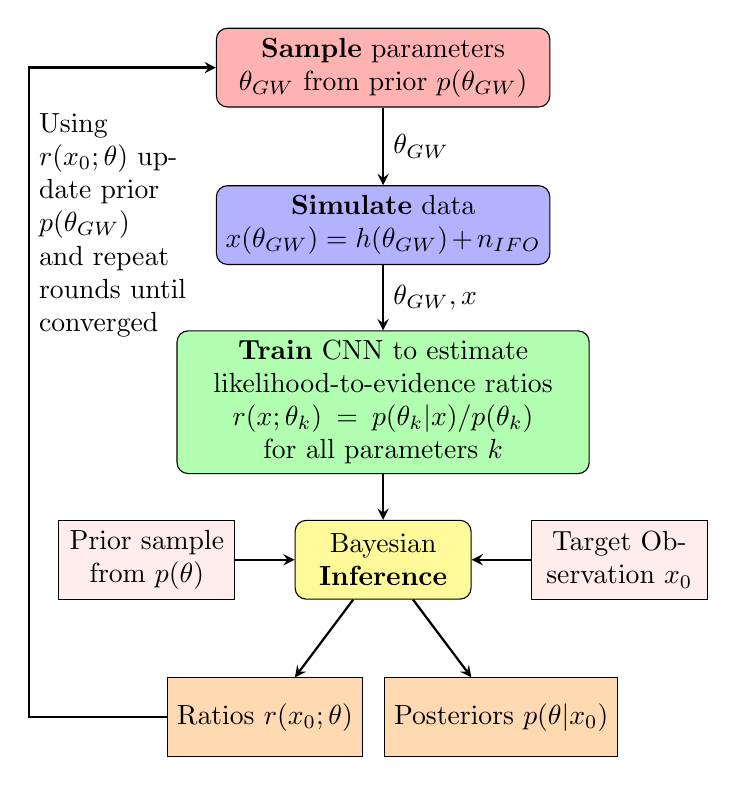
\begin{tikzpicture}[node distance=2cm]
        \node (sampling) [sample] {\textbf{Sample} parameters $\boldsymbol{\theta}_{GW}$ from prior $p(\boldsymbol{\theta}_{GW})$};
        \node (fsimulator) [simulator, below of=sampling] {\textbf{Simulate} data $\boldsymbol{x}(\theta_{GW}) = h(\theta_{GW}) + n_{IFO}$};
        \node (network) [network, below of=fsimulator, yshift=-0.25cm] {\textbf{Train} CNN to estimate likelihood-to-evidence ratios $r(\boldsymbol{x};\theta_k) = p(\theta_k|\boldsymbol{x})/p(\theta_k)$ for all parameters $k$};
        \node (inference) [inference, below of=network] {Bayesian \textbf{Inference}};
        \node (prior) [pinput, left of=inference, xshift=-1cm] {Prior sample from $p(\theta)$};
        \node (target) [tinput, right of=inference, xshift=1cm] {Target Observation $\boldsymbol{x}_0$};
        \node (ratios) [output, below of=inference, xshift=-1.5cm] {Ratios $r(\boldsymbol{x}_0;\theta)$};
        \node (posterior) [output, below of=inference, xshift=1.5cm] {Posteriors $p(\theta|\boldsymbol{x}_0)$};
        \draw [arrow] (sampling) -- node[anchor=west] {$\boldsymbol{\theta}_{GW}$} (fsimulator);
        \draw [arrow] (fsimulator) -- node[anchor=west] {$\boldsymbol{\theta}_{GW},\boldsymbol{x}$} (network);
        \draw [arrow] (network) -- (inference);
        \draw [arrow] (prior) -- (inference);
        \draw [arrow] (target) -- (inference);
        \draw [arrow] (inference) -- (posterior);
        \draw [arrow] (inference) -- (ratios);
        \draw [arrow] (ratios) -- +(-3,0) |- node[anchor=west, yshift=-2cm, text width=2cm]{Using $r(\boldsymbol{x}_0;\theta)$ update prior $p(\boldsymbol{\theta}_{GW})$ and repeat rounds until converged} (sampling);
    \end{tikzpicture}
    \caption{High-level overview of the simulation-based inference method used for this work.}
    \label{fig:peregrine_pipeline}
\end{figure}


Fifteen individual binary classifiers. Minimise binary cross-entropy loss.

Noise shuffling.

% \subsection{Optimising of sampling efficiency}

% We will investigate whether some more active learning can be introduced to increase the efficiency of the sampling process. For instance, some parameters such as the chirp mass\footnote{The chirp mass is a combination of the two object masses in the binary system, and is a key factor in the gravitational wave frequency as the two objects spiral inwards toward each other.\\$\mathcal{M} = \frac{(m_1 \cdot m_2)^{3/5}}{(m_1 + m_2)^{1/5}}$} may be inferred early on with relatively high confidence, but currently in successive simulation rounds continues to be sampled from a uniform distribution within $\pm5\sigma$~\cite{Miller_TMNRE_2021}. We will investigate whether it's possible to be more selective in the sampling of parameters that are known with relatively high confidence in an un-biased way. Therefore, we can focus the simulation budget more on the parameters we know with less confidence. To do this in a systematic way, a complete survey of how influential each parameter is on the different segments of the GW signal will be carried-out first.

The current rendition of the Peregrine pipeline requires 8 rounds of sequential TMNRE, 720000 simulated waveforms and around 12.5 hours (on a single A100 gpu with 18 cpu cores) to completely reconstruct the posteriors of the fifteen parameters. Of these 12.5 hours, around 10 is for training the network and 2.3 is for generating the waveforms used for training the network. Our primary focus is therefore the optimisation of the pipeline on the network itself, and as a secondary the number of simulated waveforms.

Trainer settings.

% ============================================================================ %
% Overview
% ============================================================================ %
\subsection{Overview of approach}

Focus on the loss 

% ============================================================================ %
% Transformer models
% ============================================================================ %
\subsection{Transformer models}



\subsubsection{Hyperparameter tuning}

RayTune was used to tune hyperparameters. 

\subsubsection{Pretraining}

Transformers were pretrained for 24 hours with single A100 gpu on 2 million waveforms.


% ============================================================================ %
% Attention U-Net
% ============================================================================ %
\subsection{Attention U-Net}



% ============================================================================ %
% Pruning
% ============================================================================ %
\subsection{Pruning}


%The architecture of the network currently implemented in \texttt{peregrine} is the U-Net architecture~\cite{Ronneberger_UNet_2015}. Given the advances in machine learning and CNN architectures since 2015, it is believed that this network can be improved upon. The optimisation of this network architecture will be the main focus of this thesis. 

%Investigative studies will be performed to find the best network architectures most suitable for the data format. We will first try with LSTM's since they are known to work well with noisy time-series data. The chosen network architecture also needs to be capable of segmenting the signal into three components, representing the different stages of the merger event -- inspiral, merger and ringdown~\cite{Pan_GW_2014}. Each of the parameters in $\boldsymbol{\theta}_{GW}$ are impacted differently in the different phases~\cite{bhardwaj2023peregrine}. Given the network is a binary classifier that classifies between joint and marginally drawn sample pairs, we will assess the performance of the network with the ROC curve.


% ============================================================================ %
% Evaluation
% ============================================================================ %
\subsection{Evaluation}

%The changes to the \texttt{peregrine} analysis pipeline will be fully benchmarked against the original \texttt{peregrine}, both in terms of accuracy of final result and required runtime. The results of the original \texttt{peregrine} have themselves been benchmarked against established likelihood-based methods~\cite{Speagle_2020}, and found to be in good agreement. Therefore, in this work we think it is sufficient to compare only with the original \texttt{peregrine}. To demonstrate the applicability of the method to real gravitational wave measurements, if time permits, we will also test the approach using real experimental data.


\section{Results}
\label{sec:results}
% Give the outcomes for each research question in the form of a table or graphic (with caption).
% Write about your results here. Good captions to tables and/or figures are key.

\subsection{Transformer models}

% Show loss curve of UNet, ViT and MVTS transformer. 
In this section, we show the results during the pretraining of the transformer models

We can conclude that the ViT does not extract any additional features from the data, since the loss plateus to the same value. However, due to extra features the ViT is much slower. The mvts model is not a good model.

The pretrained ViT model was used for the evaluation of Peregrine. Round 2 training of ViT took 11 hours, so was terminated not to waste computing budget.

AUROC for 15 features after 24 hours of training.

\begin{table}
    \caption{Loss values for each of the features}
    \begin{tabular}{lrrr}
    \toprule
    feature & mvts & vit & unet \\
    \midrule
    mass ratio & -0.231 & -0.295 & -0.300 \\
    chirp mass & -0.542 & -0.676 & -0.701 \\
    theta jn & -0.327 & -0.463 & -0.426 \\
    phase & 0.000 & 0.000 & 0.000 \\
    tilt1 & -0.107 & -0.167 & -0.174 \\
    tilt2 & -0.018 & -0.036 & -0.036 \\
    a1 & -0.078 & -0.104 & -0.132 \\
    a2 & -0.005 & -0.008 & -0.007 \\
    phi12 & 0.000 & 0.000 & 0.000 \\
    phijl & -0.199 & -0.291 & -0.287 \\
    luminosity distance & -0.196 & -0.294 & -0.291 \\
    dec & -0.830 & -0.923 & -0.899 \\
    ra & -1.020 & -1.085 & -1.066 \\
    psi & -0.063 & -0.117 & -0.090 \\
    geocent time & -0.965 & -1.104 & -1.105 \\
    \bottomrule
    \end{tabular}
\end{table}

\begin{figure}
  \centering
  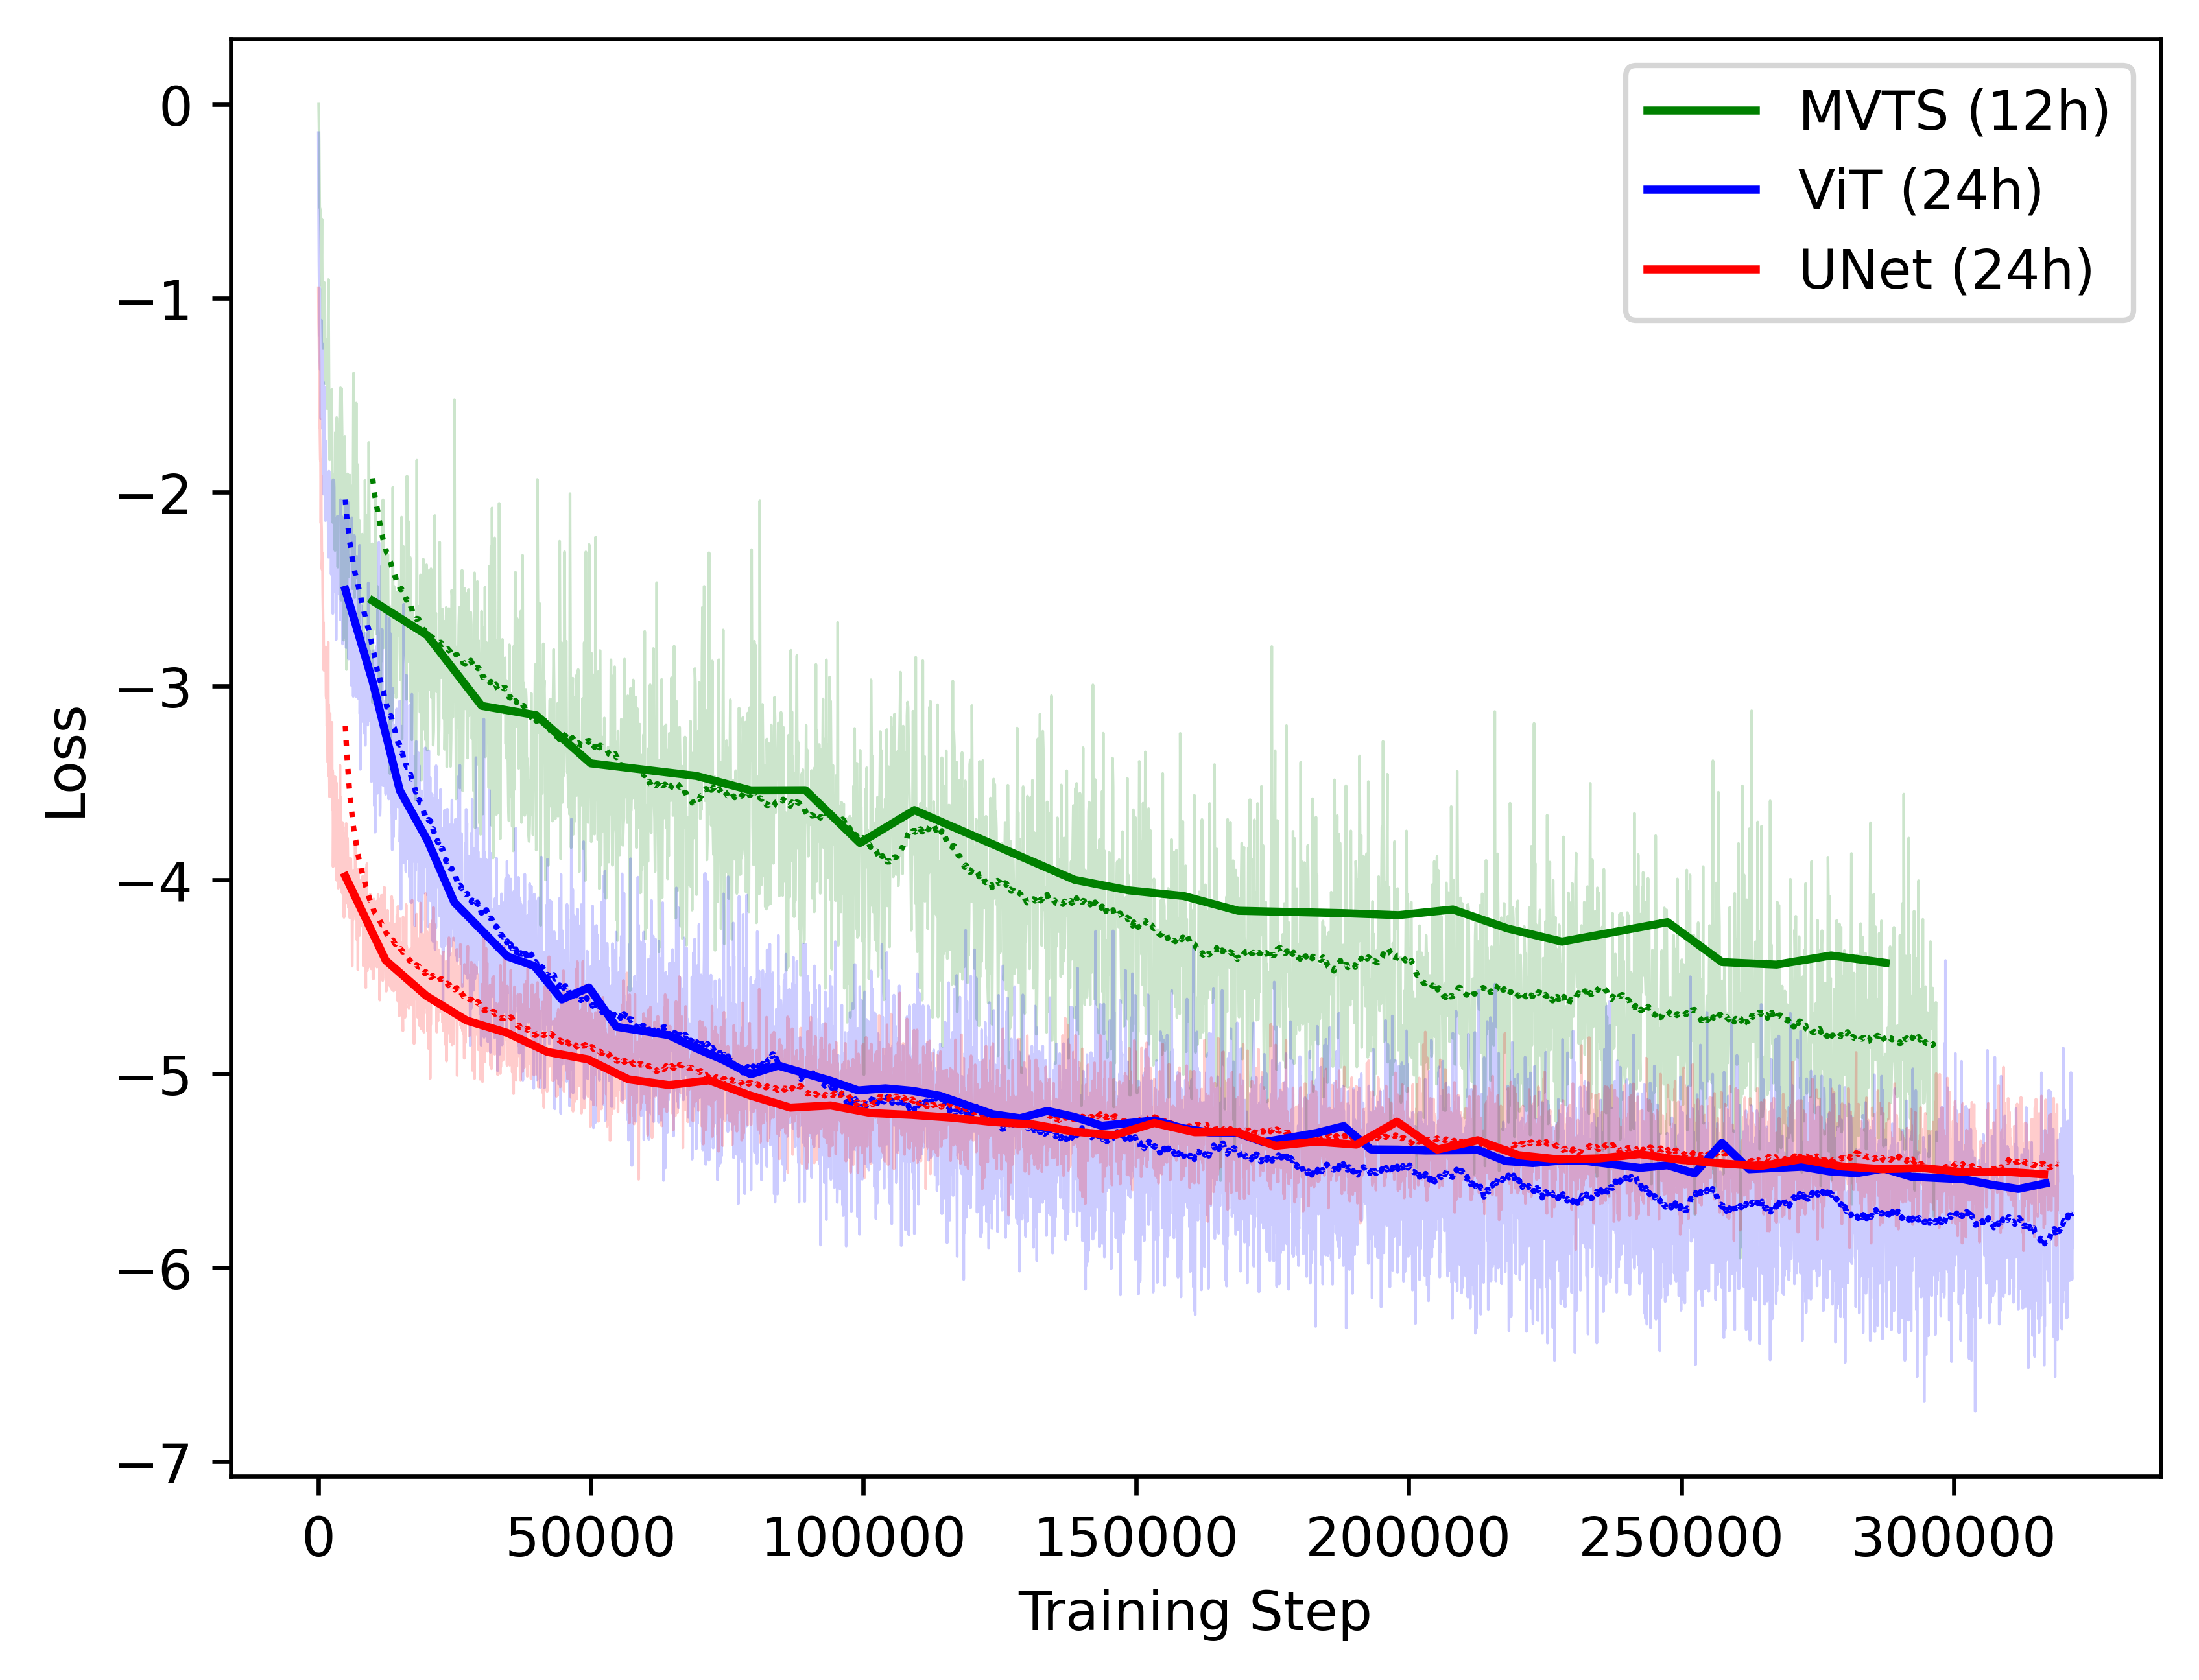
\includegraphics[width=1\linewidth]{media/images/Pretraining_loss_curve.png}
  \caption{Bla}
  \label{fig:pretain_loss_curve}
\end{figure}

\subsection{Peregrine Network}

Runtime for the rounds.

\begin{table}
\caption{Network performance of different network architectures for Peregrine}
\begin{tabular}{lrrrrrrr}
\toprule
\multicolumn{1}{p{0.5cm}}{\raggedright Network}  & 
\multicolumn{1}{p{0.5cm}}{\raggedleft Round}  &
\multicolumn{1}{p{1cm}}{\raggedleft Num \\ Epochs} &
\multicolumn{1}{p{1cm}}{\raggedleft Num \\ Steps} &
\multicolumn{1}{p{1cm}}{\raggedleft Sampling \\ Fraction} &
\multicolumn{1}{p{0.75cm}}{\raggedleft Train \\ Loss} &
\multicolumn{1}{p{0.75cm}}{\raggedleft Test \\ Loss} &
\multicolumn{1}{p{1cm}}{\raggedleft Avg \\ AUROC} \\
\midrule
UNet & 1 & 104 & 10504 & 4.98e-03 & -4.71 & -4.22 & 0.706 \\
UNet & 2 & 79 & 16432 & 2.66e-05 & -4.78 & -4.65 & 0.738 \\
UNet & 3 & 77 & 23793 & 2.38e-06 & -4.71 & -4.47 & 0.741 \\
UNet & 4 & 74 & 30858 & 1.61e-06 & -4.14 & -4.43 & 0.741 \\
UNet & 5 & 90 & 37530 & 8.15e-07 & -4.43 & -4.39 & 0.742 \\
UNet & 6 & 60 & 31440 & 6.03e-07 & -4.19 & -4.25 & 0.736 \\
\midrule
Att UNet & 1 & 74 & 7474 & 1.04e-02 & -4.48 & -4.16 & 0.710 \\
Att UNet & 2 & 78 & 16224 & 2.21e-05 & -4.83 & -4.65 & 0.731 \\
Att UNet & 3 & 58 & 17922 & 5.59e-06 & -4.35 & -4.35 & 0.735 \\
Att UNet & 4 & 54 & 22518 & 2.76e-06 & -4.32 & -4.27 & 0.736 \\
Att UNet & 5 & 87 & 36279 & 2.51e-06 & -4.38 & -4.16 & 0.735 \\
Att UNet & 6 & 83 & 43492 & 1.74e-06 & -4.09 & -4.19 & 0.734 \\
\midrule
UNet 5\% & 1 & 68 & 6868 & 4.21e-03 & -5.03 & -4.43 & 0.716 \\
UNet 5\% & 2 & 65 & 13520 & 5.40e-05 & -4.85 & -4.49 & 0.731 \\
UNet 5\% & 3 & 75 & 23175 & 7.71e-06 & -4.05 & -4.33 & 0.736 \\
UNet 5\% & 4 & 48 & 20016 & 4.67e-06 & -4.09 & -4.41 & 0.743 \\
UNet 5\% & 5 & 60 & 25020 & 3.91e-06 & -4.27 & -4.46 & 0.743 \\
UNet 5\% & 6 & 30 & 15720 & 3.52e-06 & -4.74 & -4.38 & 0.741 \\
\midrule
UNet 10\% & 1 & 39 & 3939 & 4.31e-02 & -3.98 & -3.89 & 0.689 \\
UNet 10\% & 2 & 35 & 7280 & 3.72e-03 & -3.67 & -3.76 & 0.706 \\
UNet 10\% & 3 & 58 & 17922 & 4.33e-05 & -4.42 & -4.62 & 0.732 \\
UNet 10\% & 4 & 57 & 23769 & 1.14e-05 & -4.54 & -4.27 & 0.735 \\
UNet 10\% & 5 & 30 & 12510 & 8.17e-06 & -3.90 & -3.96 & 0.725 \\
UNet 10\% & 6 & 56 & 29344 & 4.87e-06 & -4.08 & -4.31 & 0.738 \\
\midrule
ViT & 1 & 30 & 12540 & 4.37e-05 & -6.15 & -5.58 & 0.753 \\
ViT & 2 & 60 & 50460 & 2.03e-06 & -5.82 & -5.28 & 0.757 \\
\bottomrule
\end{tabular}
\end{table}


Look at different parameters for round 6.
Compare the four different UNet models.

\begin{table}
\caption{Round 6 AUC and loss values}
\hspace*{-2cm}
\begin{tabular}{lrrrrrrrr}
\toprule
Param & 
\multicolumn{1}{p{0.3cm}}{\raggedright UNet}  & 
\multicolumn{1}{p{0.3cm}}{\raggedleft Att UNet}  &
\multicolumn{1}{p{0.3cm}}{\raggedleft UNet 10\%}  &
\multicolumn{1}{p{0.3cm}}{\raggedleft UNet 5\%}  &
\multicolumn{1}{p{0.3cm}}{\raggedright UNet}  & 
\multicolumn{1}{p{0.3cm}}{\raggedleft Att UNet}  &
\multicolumn{1}{p{0.3cm}}{\raggedleft UNet 10\%}  &
\multicolumn{1}{p{0.3cm}}{\raggedleft UNet 5\%}  \\
\midrule
\( q \) & 0.765 & 0.756 & 0.744 & 0.761 & -0.282 & -0.257 & -0.246 & -0.275 \\
\( M \) & 0.833 & 0.817 & 0.825 & 0.817 & -0.448 & -0.403 & -0.428 & -0.415 \\
\( \theta_{jn} \) & 0.800 & 0.795 & 0.815 & 0.812 & -0.352 & -0.343 & -0.391 & -0.386 \\
\( \phi_c \) & 0.499 & 0.500 & 0.501 & 0.506 & 0.000 & 0.000 & 0.000 & -0.000 \\
\( \theta_1 \) & 0.756 & 0.754 & 0.746 & 0.748 & -0.243 & -0.240 & -0.221 & -0.226 \\
\( \theta_2 \) & 0.638 & 0.640 & 0.627 & 0.628 & -0.069 & -0.069 & -0.055 & -0.058 \\
\( a_1 \) & 0.725 & 0.714 & 0.715 & 0.722 & -0.193 & -0.180 & -0.170 & -0.187 \\
\( a_2 \) & 0.573 & 0.571 & 0.567 & 0.579 & -0.022 & -0.023 & -0.019 & -0.023 \\
\( \phi_{12} \) & 0.499 & 0.498 & 0.502 & 0.503 & 0.000 & 0.001 & 0.000 & -0.000 \\
\( \phi_{jl} \) & 0.856 & 0.892 & 0.890 & 0.901 & -0.503 & -0.620 & -0.594 & -0.633 \\
\( d_L \) & 0.828 & 0.812 & 0.814 & 0.818 & -0.444 & -0.400 & -0.394 & -0.411 \\
\( \delta \) & 0.848 & 0.846 & 0.856 & 0.859 & -0.496 & -0.480 & -0.506 & -0.519 \\
\( \alpha \) & 0.858 & 0.841 & 0.854 & 0.853 & -0.520 & -0.468 & -0.509 & -0.501 \\
\( \psi \) & 0.714 & 0.715 & 0.741 & 0.746 & -0.175 & -0.177 & -0.217 & -0.231 \\
\( t_c \) & 0.854 & 0.865 & 0.873 & 0.854 & -0.515 & -0.545 & -0.565 & -0.511 \\

\bottomrule
\end{tabular}
\end{table}

\subsection{Peregrine Run Strategy}

% Network reinitialisation
% Sampling strategy
% Simulation scheduling

% Compare posteriors of 

% Sometimes,  especially  if  you  have  quite  different experiments or research  questions,  it makes sense to interleave the experimental setup and the results sections, so the reader does not get lost. It is then helpful to structure clearly in (sub)subsections.
\section{Discussion}
\label{sec:discussion}
% Compare your results with the state-of-the-art and reflect upon the results and limitations of the study. You can already hint at future work to which you come back in the conclusion section.
Write your discussion here. Do not forget to use sub-sections. Normally, the discussion starts with comparing your results to other studies as precisely as possible. The limitations should be reflected upon in terms such as reproducibility,  scalability,  generalizability,  reliability  and  validity. It is also important to mention ethical concerns.
\section{Conclusion}
\label{sec:conclusion}
% Answer each research question and address how the limitations of the study qualify the conclusion.
Write your conclusion here. Be sure that the relation between the research gap and your contribution is clear. Be honest about how limitations in the study qualify the answer on the research question.

\bibliographystyle{ACM-Reference-Format}
\bibliography{bibliographies/references}

\newpage
% You can choose whether you prefer a single or double column appendix.
% Whatever you choose, you will need to stick to it throughout the appendix.
% For double column style, comment the next line.
\onecolumn

\appendix
\begin{appendices}

\section{Posterior Plots}
\label{sec:apx:posterior_plots}

\begin{figure}[htb]
  \centering
  \includegraphics[width=0.85\linewidth]{media/images/Posteriors_UNet_original_half_round_8.png}
  \caption{Comparison between U-Net (blue) and U-Net with half the number of simulations (red) after 8 rounds of TMNRE.}
  \label{fig:posterior_unet_half}
  \Description[<short description>]{<long description>}
\end{figure}

\begin{figure}[htb]
  \centering
  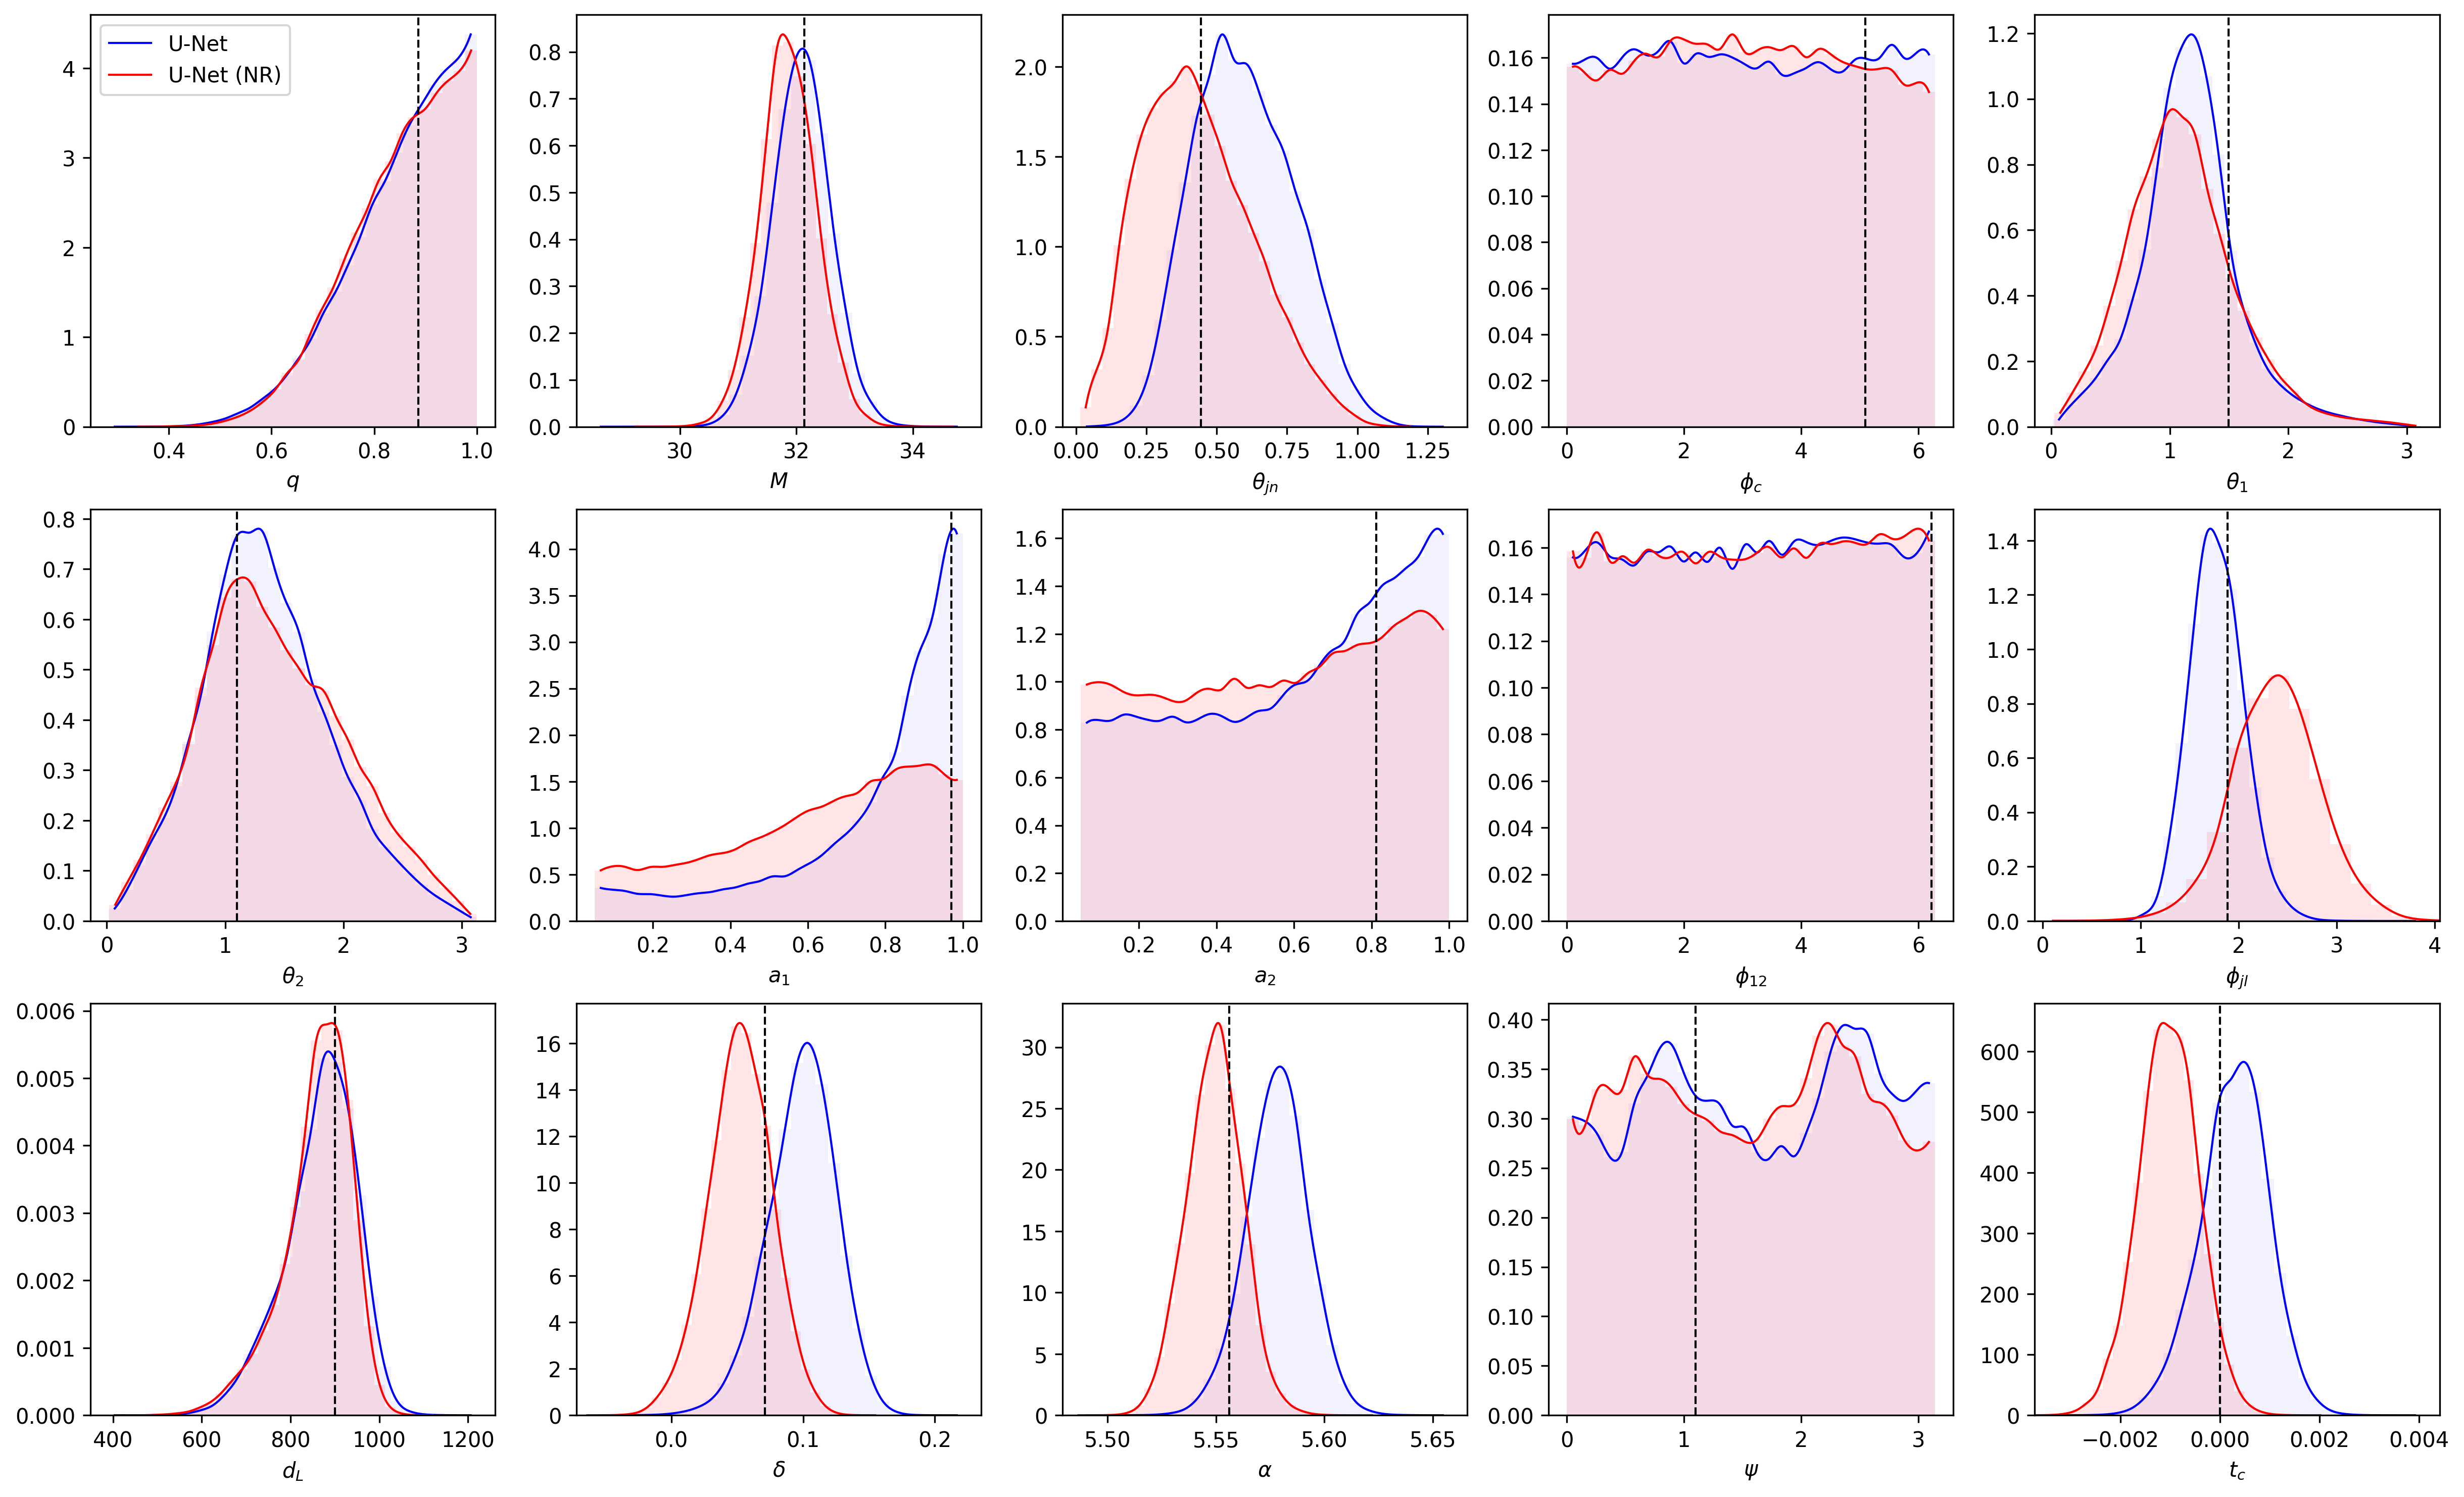
\includegraphics[width=0.85\linewidth]{media/images/Posteriors_UNet_NoReinit_round_8.png}
  \caption{Comparison between U-Net (blue) and U-Net with no re-initialisation (red) after 8 rounds of TMNRE.}
  \label{fig:posterior_unet_noreinit}
  \Description[<short description>]{<long description>}
\end{figure}

\begin{figure}[htb]
  \centering
  \includegraphics[width=0.85\linewidth]{media/images/Posteriors_AttentionUNet_2_round_8.png}
  \caption{Comparison between U-Net (blue) and Attention U-Net (red) after 8 rounds of TMNRE.}
  \label{fig:posterior_attention_unet}
  \Description[<short description>]{<long description>}
\end{figure}

\begin{figure}[htb]
  \centering
  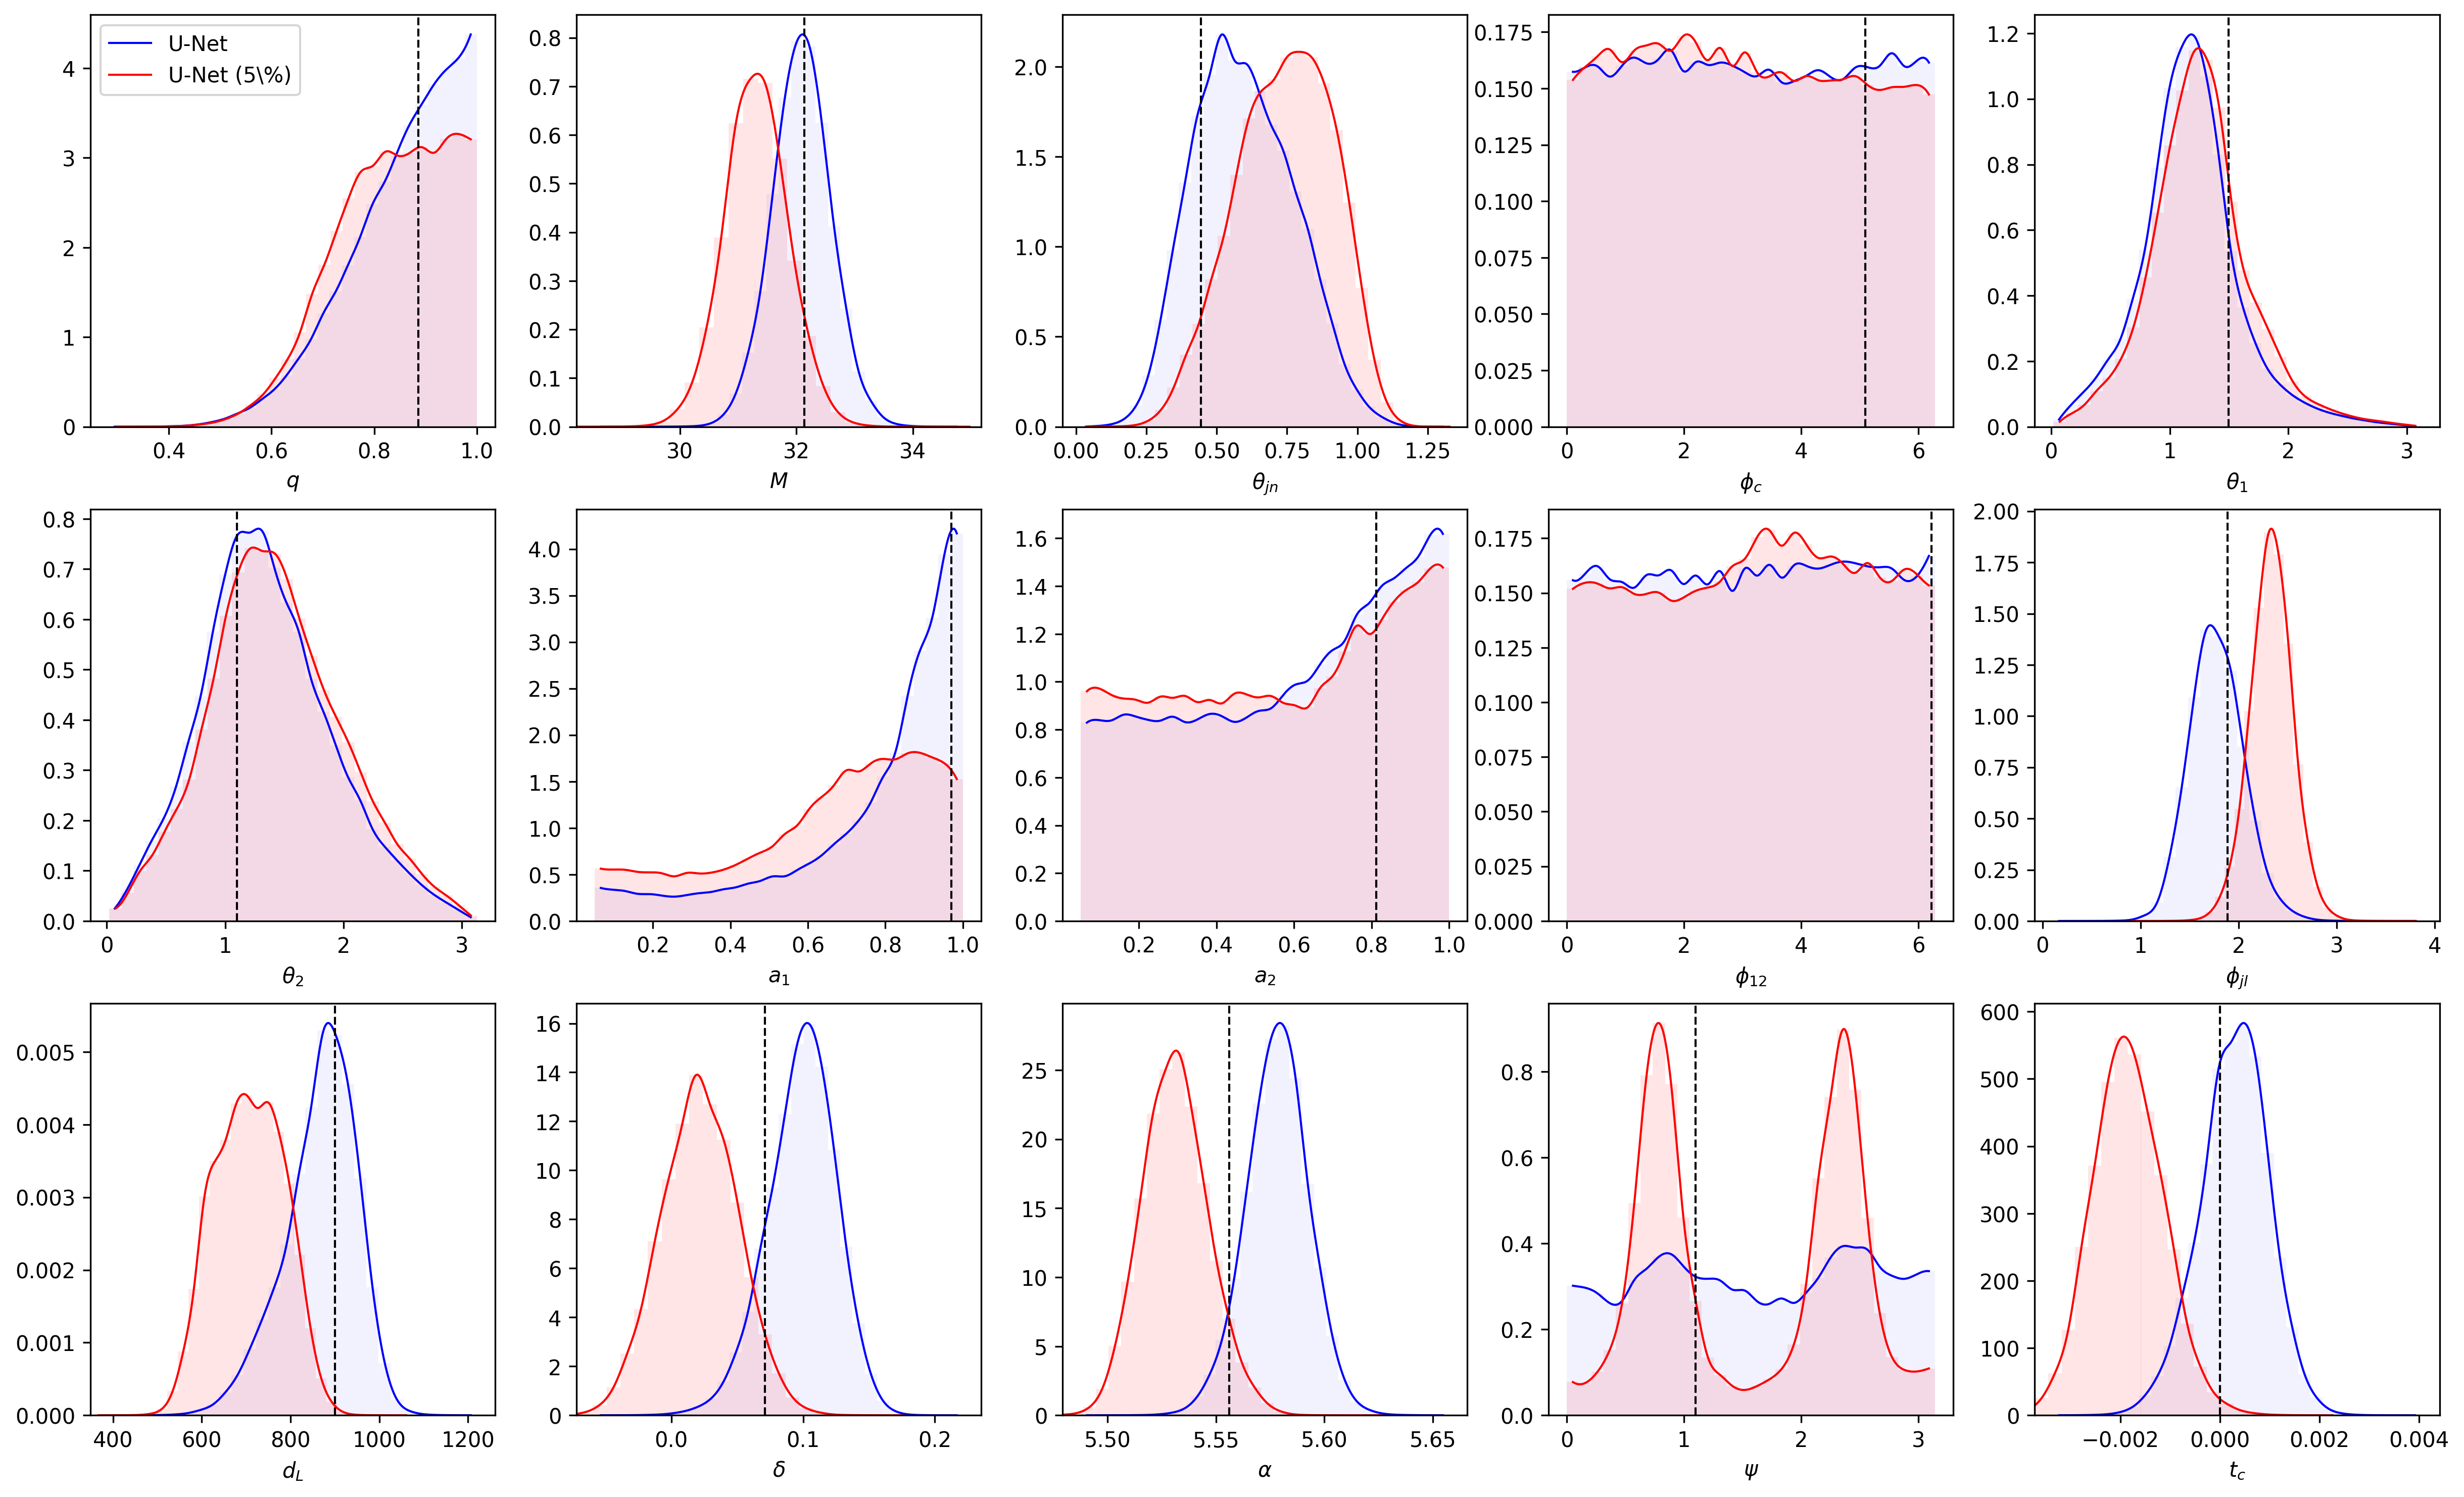
\includegraphics[width=0.85\linewidth]{media/images/Posteriors_UNet_pruned5_2_round_8.png}
  \caption{Comparison between U-Net (blue) and U-Net 5\% pruned (red) after 8 rounds of TMNRE.}
  \label{fig:posterior_unet_pruned_5pc}
  \Description[<short description>]{<long description>}
\end{figure}

\begin{figure}[htb]
  \centering
  \includegraphics[width=0.85\linewidth]{media/images/Posteriors_UNet_pruned10_round_8.png}
  \caption{Comparison between U-Net (blue) and U-Net 10\% pruned (red) after 8 rounds of TMNRE.}
  \label{fig:posterior_unet_pruned_10pc}
  \Description[<short description>]{<long description>}
\end{figure}

\begin{figure}[htb]
  \centering
  \includegraphics[width=0.85\linewidth]{media/images/Posteriors_ViT_pretrained_2_round_3.png}
  \caption{Comparison between U-Net (blue) and ViT transformer (red) after 3 rounds of TMNRE.}
  \label{fig:posterior_vit}
  \Description[<short description>]{<long description>}
\end{figure}

\FloatBarrier

\section{U-Net}
\label{sec:apx:u-net_architecture}

\begin{figure}[htb]
	\centering
	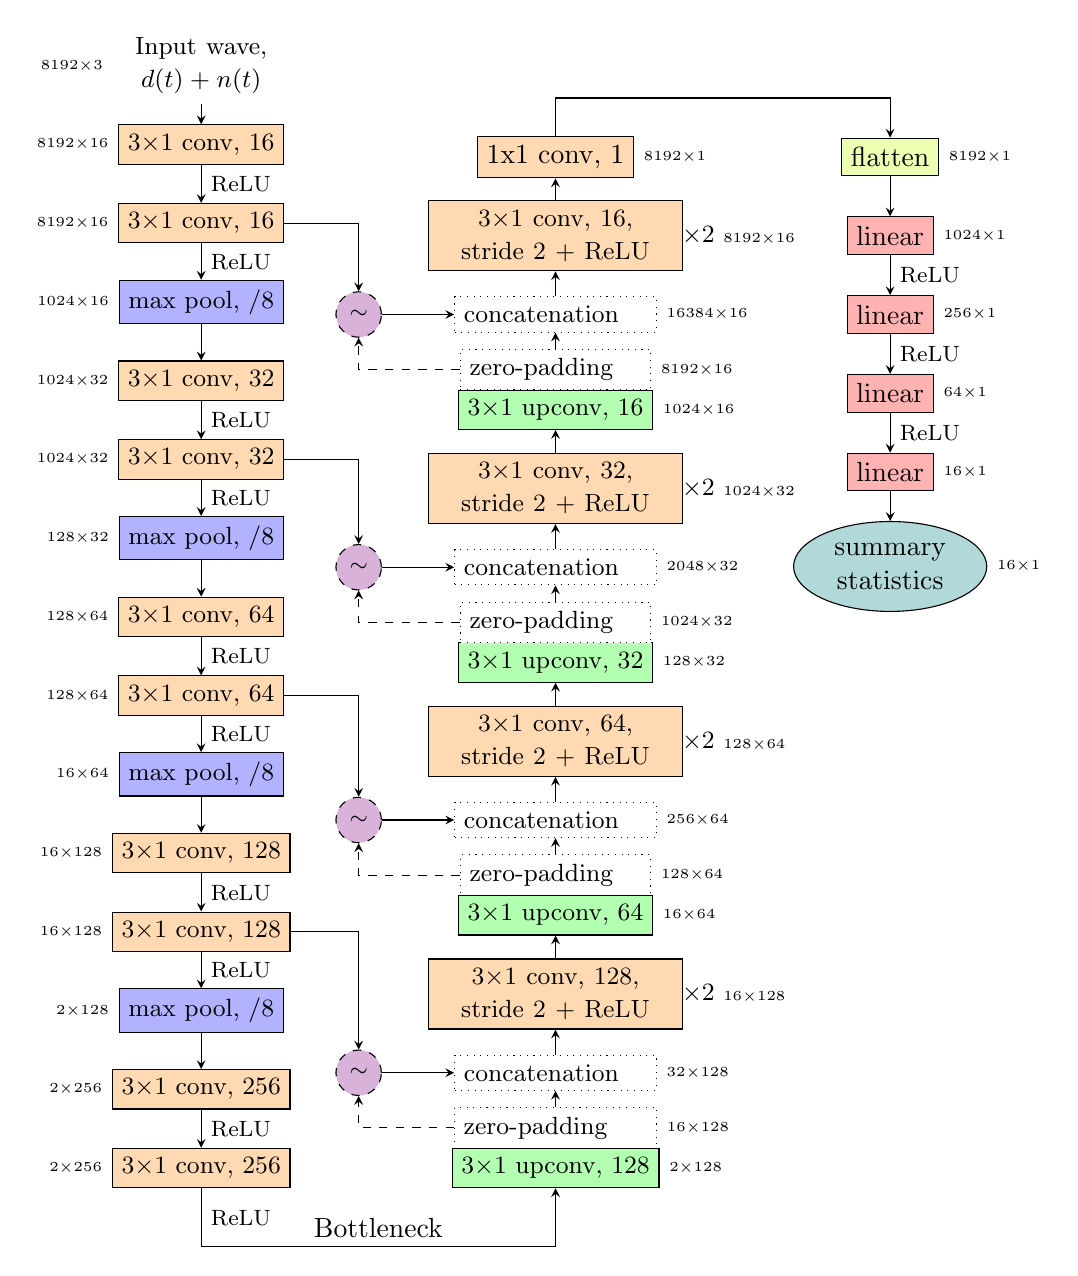
\begin{tikzpicture}[node distance=1.0cm]
		
    %%% NODES
    
    \node (input) [input, label=west:\tiny 8192$\times$3, text width=2cm] {\small Input wave, $d(t)+n(t)$};

    \node (conv1) [conv, below of=input, label=west:\tiny 8192$\times$16] {\small 3$\times$1 conv, 16};
    \node (conv2) [conv, below of=conv1, label=west:\tiny 8192$\times$16] {\small 3$\times$1 conv, 16};
    
    \node (pool1) [pool, below of=conv2, label=west:\tiny 1024$\times$16] {\small max pool, /8};
    
    \node (conv3) [conv, below of=pool1, label=west:\tiny 1024$\times$32] {\small 3$\times$1 conv, 32};
    \node (conv4) [conv, below of=conv3, label=west:\tiny 1024$\times$32] {\small 3$\times$1 conv, 32};
    
    \node (pool2) [pool, below of=conv4, label=west:\tiny 128$\times$32] {\small max pool, /8};
    
    \node (conv5) [conv, below of=pool2, label=west:\tiny 128$\times$64] {\small 3$\times$1 conv, 64};
    \node (conv6) [conv, below of=conv5, label=west:\tiny 128$\times$64] {\small 3$\times$1 conv, 64};
    
    \node (pool3) [pool, below of=conv6, label=west:\tiny 16$\times$64] {\small max pool, /8};
    
    \node (conv7) [conv, below of=pool3, label=west:\tiny 16$\times$128] {\small 3$\times$1 conv, 128};
    \node (conv8) [conv, below of=conv7, label=west:\tiny 16$\times$128] {\small 3$\times$1 conv, 128};
    
    \node (pool4) [pool, below of=conv8, label=west:\tiny 2$\times$128] {\small max pool, /8};

    \node (conv9) [conv, below of=pool4, label=west:\tiny 2$\times$256] {\small 3$\times$1 conv, 256};
    \node (conv10) [conv, below of=conv9, label=west:\tiny 2$\times$256] {\small 3$\times$1 conv, 256};
    
    %%%%%
    
    \node (upconv1) [upconv, right of=conv10, label=east:\tiny 2$\times$128, xshift=3.5cm] {\small 3$\times$1 upconv, 128};
    \node (zp1) [concat, above of=upconv1, label=east:\tiny 16$\times$128, yshift=-0.49cm] {\small zero-padding \hspace{0.4cm} };
    \node (concat1) [concat, above of=zp1, label=east:\tiny 32$\times$128, yshift=-0.3cm] {\small concatenation \hspace{0.25cm} };
    \node (upconvrelu1) [convx2, text width=3cm, above of=concat1, label=east:\small \hspace{-0.25cm} $\times$2 \tiny 16$\times$128] {\small 3$\times$1 conv, 128, stride 2 + ReLU};
    
    \node (AG1) [AG, left of=concat1, xshift=-1.5cm] {\footnotesize $\sim$};

    \node (upconv2) [upconv, above of=upconvrelu1, label=east:\tiny 16$\times$64] {\small 3$\times$1 upconv, 64};
    \node (zp2) [concat, above of=upconv2, label=east:\tiny 128$\times$64, yshift=-0.49cm] {\small zero-padding \hspace{0.25cm} };
    \node (concat2) [concat, above of=zp2, label=east:\tiny 256$\times$64, yshift=-0.3cm] {\small concatenation \hspace{0.25cm} };
    \node (upconvrelu2) [convx2, text width=3cm, above of=concat2, label=east:\small \hspace{-0.25cm} $\times$2 \tiny 128$\times$64] {\small 3$\times$1 conv, 64, stride 2 + ReLU};
    
    \node (AG2) [AG, left of=concat2, xshift=-1.5cm] {\footnotesize $\sim$};

    \node (upconv3) [upconv, above of=upconvrelu2, label=east:\tiny 128$\times$32] {\small 3$\times$1 upconv, 32};
    \node (zp3) [concat, above of=upconv3, label=east:\tiny 1024$\times$32, yshift=-0.49cm] {\small zero-padding \hspace{0.25cm} };
    \node (concat3) [concat, above of=zp3, label=east:\tiny 2048$\times$32, yshift=-0.3cm] {\small concatenation \hspace{0.25cm} };
    \node (upconvrelu3) [convx2, text width=3cm, above of=concat3, label=east:\small \hspace{-0.25cm} $\times$2 \tiny 1024$\times$32] {\small 3$\times$1 conv, 32, stride 2 + ReLU};
    
    \node (AG3) [AG, left of=concat3, xshift=-1.5cm] {\footnotesize $\sim$};
    
    \node (upconv4) [upconv, above of=upconvrelu3, label=east:\tiny 1024$\times$16] {\small 3$\times$1 upconv, 16};
    \node (zp4) [concat, above of=upconv4, label=east:\tiny 8192$\times$16, yshift=-0.49cm] {\small zero-padding \hspace{0.25cm} };
    \node (concat4) [concat, above of=zp4, label=east:\tiny 16384$\times$16, yshift=-0.3cm] {\small concatenation \hspace{0.25cm} };
    \node (upconvrelu4) [convx2, text width=3cm, above of=concat4, label=east:\small \hspace{-0.25cm} $\times$2 \tiny 8192$\times$16] {\small 3$\times$1 conv, 16, stride 2 + ReLU};
    
    \node (AG4) [AG, left of=concat4, xshift=-1.5cm] {\footnotesize $\sim$};

    \node (outconv) [outconv, above of=upconvrelu4, label=east:\tiny 8192$\times$1] {1x1 conv, 1};
    
    %%%
    
    \node (flatten) [flatten, right of=outconv, label=east:\tiny 8192$\times$1, xshift=3.25cm] {flatten};
    \node (fc1) [fc, below of=flatten, label=east:\tiny 1024$\times$1] {linear};
    \node (fc2) [fc, below of=fc1, label=east:\tiny 256$\times$1] {linear};
    \node (fc3) [fc, below of=fc2, label=east:\tiny 64$\times$1] {linear};
    \node (fc4) [fc, below of=fc3, label=east:\tiny 16$\times$1] {linear};
    \node (summary) [summary, below of=fc4, label=east:\tiny 16$\times$1, yshift=-0.2cm] {summary statistics};
    
    %%% EDGES
                
    \draw [arrow_unet] (input) -- node[anchor=west]{}(conv1);
    
    \draw [arrow_unet] (conv1) -- node[anchor=west]{\footnotesize ReLU}(conv2);
    \draw [arrow_unet] (conv2) -- node[anchor=west]{\footnotesize ReLU}(pool1);
    \draw [arrow_unet] (pool1) -- node[anchor=west]{}(conv3);
    \draw [arrow_unet] (conv3) -- node[anchor=west]{\footnotesize ReLU}(conv4);
    \draw [arrow_unet] (conv4) -- node[anchor=west]{\footnotesize ReLU}(pool2);
    \draw [arrow_unet] (pool2) -- node[anchor=west]{}(conv5);
    \draw [arrow_unet] (conv5) -- node[anchor=west]{\footnotesize ReLU}(conv6);
    \draw [arrow_unet] (conv6) -- node[anchor=west]{\footnotesize ReLU}(pool3);
    \draw [arrow_unet] (pool3) -- node[anchor=west]{}(conv7);
    \draw [arrow_unet] (conv7) -- node[anchor=west]{\footnotesize ReLU}(conv8);
    \draw [arrow_unet] (conv8) -- node[anchor=west]{\footnotesize ReLU}(pool4);
    \draw [arrow_unet] (pool4) -- node[anchor=west]{}(conv9);
    \draw [arrow_unet] (conv9) -- node[anchor=west]{\footnotesize ReLU}(conv10);
    
    \draw [arrow_unet] (conv10) -- +(0,-1) node[pos=0.5, right]{\footnotesize ReLU} -| node[pos=0.25, above]{Bottleneck}(upconv1);
    
    %%%
    
    \draw [arrow_unet_dotted] (zp1) -| node[anchor=east]{}(AG1);			
    \draw [arrow_unet] (conv8) -| node[anchor=west]{}(AG1);
    \draw [arrow_unet] (AG1) -- node[anchor=west]{}(concat1);
    
    \draw [arrow_unet] (zp1) -- node[anchor=west]{}(concat1);
    \draw [arrow_unet] (concat1) -- node[anchor=west]{}(upconvrelu1);			
    \draw [arrow_unet] (upconvrelu1) -- node[anchor=west]{}(upconv2);			
    
    \draw [arrow_unet_dotted] (zp2) -| node[anchor=east]{}(AG2);			
    \draw [arrow_unet] (conv6) -| node[anchor=west]{}(AG2);
    \draw [arrow_unet] (AG2) -- node[anchor=west]{}(concat2);
    
    \draw [arrow_unet] (zp2) -- node[anchor=west]{}(concat2);
    \draw [arrow_unet] (concat2) -- node[anchor=west]{}(upconvrelu2);			
    \draw [arrow_unet] (upconvrelu2) -- node[anchor=west]{}(upconv3);	
    
    \draw [arrow_unet_dotted] (zp3) -| node[anchor=east]{}(AG3);			
    \draw [arrow_unet] (conv4) -| node[anchor=west]{}(AG3);
    \draw [arrow_unet] (AG3) -- node[anchor=west]{}(concat3);
    
    \draw [arrow_unet] (zp3) -- node[anchor=west]{}(concat3);
    \draw [arrow_unet] (concat3) -- node[anchor=west]{}(upconvrelu3);			
    \draw [arrow_unet] (upconvrelu3) -- node[anchor=west]{}(upconv4);	
    
    \draw [arrow_unet_dotted] (zp4) -| node[anchor=east]{}(AG4);			
    \draw [arrow_unet] (conv2) -| node[anchor=west]{}(AG4);
    \draw [arrow_unet] (AG4) -- node[anchor=west]{}(concat4);
    
    \draw [arrow_unet] (zp4) -- node[anchor=west]{}(concat4);
    \draw [arrow_unet] (concat4) -- node[anchor=west]{}(upconvrelu4);			
    \draw [arrow_unet] (upconvrelu4) -- node[anchor=west]{}(outconv);	
    
    %%%
    
    \draw [arrow_unet] (outconv) -- +(0,0.75) -| node[anchor=west]{}(flatten);
    \draw [arrow_unet] (flatten) -- node[anchor=west]{}(fc1);
    \draw [arrow_unet] (fc1) -- node[anchor=west]{\footnotesize ReLU}(fc2);
    \draw [arrow_unet] (fc2) -- node[anchor=west]{\footnotesize ReLU}(fc3);
    \draw [arrow_unet] (fc3) -- node[anchor=west]{\footnotesize ReLU}(fc4);
    \draw [arrow_unet] (fc4) -- node[anchor=west]{}(summary);
			
	\end{tikzpicture}	
 
\caption{The architecture of (Attention) U-Net as implemented for the processing of the time domain signal. The frequency domain follows the same architecture, but the max pooling layer is a factor of 2, and the initial input wave is 4097$\times$6. Left column shows the encoder stage, middle column shows the decoder stage, and the right column shows the linear compression performed in Peregrine to reduce the U-Net output into the summary statistics. The difference between Attention U-Net and original U-Net is the addition of the Attention gates ($\sim$) in the skip layers (indicated with dashed lines).}
\label{fig:Attention_UNet_arch}
 \end{figure}

\section{Hyperparameter tuning}
\label{sec:apx:Hyperparameter_tuning}

Hyperparameters for the ViT transformer models were first tuned for the time domain and frequency domain signals separately. Once the optimal hyperparameters for those had been found, an additional step of combining the two models to find the optimal number of classes for each was performed. The dimensions of the MLP was also reassessed to ensure consistency. Results are given in Tables~\ref{tab:hyperparams_vit_t}, \ref{tab:hyperparams_vit_f}, and \ref{tab:hyperparams_vit_combined}.

Results for the hyperparameter tuning of the MTS transformer models is given in Table~\ref{tab:hyperparams_mts}. Due to the optimal hyperparameters of the ViT model for the time and frequency networks being the same, the MTS network was tuned with the time and frequency networks together. The number of classes and patch size was also fixed at 16.

\begin{table}
\caption{Different trials for the hyperparameter tuning of the ViT transformer for the time domain signal. In total there were 69 trials performed, but only the 10 best and 10 worst trials are shown.}
\label{tab:hyperparams_vit_t}
\begin{tabular}{rrrrrrrrrrrrr}
\toprule
\multicolumn{1}{p{0.5cm}}{\raggedleft Batch size} & 
\multicolumn{1}{p{0.5cm}}{\raggedleft Depth} & 
\multicolumn{1}{p{1.0cm}}{\raggedleft Dimen-sions} & 
\multicolumn{1}{p{1.0cm}}{\raggedleft Dropout} & 
\multicolumn{1}{p{1.0cm}}{\raggedleft EMB dropout} & 
\multicolumn{1}{p{1.0cm}}{\raggedleft Num heads} & 
\multicolumn{1}{p{0.5cm}}{\raggedleft LR} & 
\multicolumn{1}{p{0.5cm}}{\raggedleft MLP dim} & 
\multicolumn{1}{p{1.0cm}}{\raggedleft Num classes} & 
\multicolumn{1}{p{1.0cm}}{\raggedleft Patch size} & 
\multicolumn{1}{p{1.0cm}}{\raggedleft Epochs} & 
\multicolumn{1}{p{1.5cm}}{\raggedleft Time per epoch (s)} & 
\multicolumn{1}{p{0.5cm}}{\raggedleft Loss} \\
\midrule
64 & 7 & 512 & 0.00 & 0.00 & 7 & 1.60e-04 & 1024 & 16 & 16 & 20 & 125 & -2.81 \\
64 & 7 & 512 & 0.00 & 0.00 & 6 & 1.60e-04 & 1024 & 24 & 16 & 20 & 114 & -2.80 \\
64 & 7 & 512 & 0.00 & 0.00 & 6 & 1.60e-04 & 1024 & 32 & 16 & 20 & 116 & -2.79 \\
64 & 7 & 512 & 0.00 & 0.00 & 6 & 1.60e-04 & 2048 & 24 & 16 & 17 & 146 & -2.64 \\
64 & 7 & 512 & 0.00 & 0.00 & 6 & 1.20e-04 & 2048 & 24 & 16 & 10 & 148 & -2.41 \\
32 & 7 & 1024 & 0.00 & 0.10 & 7 & 1.20e-04 & 1024 & 16 & 16 & 10 & 199 & -2.33 \\
64 & 6 & 512 & 0.00 & 0.10 & 8 & 1.60e-04 & 1024 & 32 & 16 & 10 & 119 & -2.32 \\
64 & 7 & 512 & 0.00 & 0.00 & 7 & 1.60e-04 & 1024 & 32 & 16 & 7 & 125 & -2.20 \\
64 & 7 & 512 & 0.00 & 0.00 & 8 & 1.60e-04 & 1024 & 24 & 16 & 7 & 135 & -2.20 \\
64 & 7 & 512 & 0.00 & 0.00 & 6 & 1.60e-04 & 1024 & 16 & 16 & 7 & 115 & -2.19 \\
\midrule
32 & 5 & 1024 & 0.20 & 0.00 & 10 & 1.20e-04 & 1024 & 28 & 16 & 1 & 185 & -0.73 \\
64 & 10 & 512 & 0.20 & 0.00 & 10 & 1.20e-04 & 1024 & 24 & 16 & 1 & 232 & -0.71 \\
32 & 5 & 2048 & 0.00 & 0.00 & 7 & 1.20e-04 & 1024 & 24 & 8 & 1 & 504 & -0.59 \\
32 & 4 & 256 & 0.10 & 0.00 & 7 & 1.20e-04 & 2048 & 16 & 8 & 1 & 190 & -0.58 \\
32 & 8 & 2048 & 0.10 & 0.20 & 6 & 1.20e-04 & 2048 & 20 & 8 & 1 & 1048 & -0.47 \\
32 & 8 & 2048 & 0.00 & 0.00 & 9 & 1.60e-04 & 2048 & 24 & 8 & 1 & 1192 & -0.44 \\
32 & 7 & 1024 & 0.20 & 0.10 & 8 & 1.60e-04 & 1024 & 28 & 8 & 1 & 506 & -0.42 \\
32 & 9 & 512 & 0.20 & 0.00 & 8 & 1.20e-04 & 2048 & 28 & 8 & 1 & 565 & -0.42 \\
32 & 10 & 1024 & 0.20 & 0.00 & 6 & 1.60e-04 & 2048 & 16 & 8 & 1 & 782 & -0.37 \\
32 & 4 & 256 & 0.20 & 0.20 & 9 & 1.60e-04 & 1024 & 32 & 8 & 1 & 200 & -0.33 \\
\bottomrule
\end{tabular}
\end{table}

\begin{table}
\caption{Different trials for the hyperparameter tuning of the ViT transformer for the frequency domain signal. In total there were 77 trials performed, but only the 10 best and 10 worst trials are shown.}
\label{tab:hyperparams_vit_f}
\begin{tabular}{rrrrrrrrrrrrr}
\toprule
\multicolumn{1}{p{0.5cm}}{\raggedleft Batch size} & 
\multicolumn{1}{p{0.5cm}}{\raggedleft Depth} & 
\multicolumn{1}{p{1.0cm}}{\raggedleft Dimen-sions} & 
\multicolumn{1}{p{1.0cm}}{\raggedleft Dropout} & 
\multicolumn{1}{p{1.0cm}}{\raggedleft EMB dropout} & 
\multicolumn{1}{p{1.0cm}}{\raggedleft Num heads} & 
\multicolumn{1}{p{0.5cm}}{\raggedleft LR} & 
\multicolumn{1}{p{0.5cm}}{\raggedleft MLP dim} & 
\multicolumn{1}{p{1.0cm}}{\raggedleft Num classes} & 
\multicolumn{1}{p{1.0cm}}{\raggedleft Patch size} & 
\multicolumn{1}{p{1.0cm}}{\raggedleft Epochs} & 
\multicolumn{1}{p{1.5cm}}{\raggedleft Time per epoch (s)} & 
\multicolumn{1}{p{0.5cm}}{\raggedleft Loss} \\
\midrule
64 & 7 & 512 & 0.00 & 0.00 & 6 & 1.60e-04 & 2048 & 24 & 16 & 20 & 74 & -2.64 \\
128 & 5 & 1024 & 0.05 & 0.00 & 7 & 1.97e-04 & 1024 & 24 & 16 & 20 & 70 & -2.59 \\
128 & 6 & 512 & 0.05 & 0.10 & 8 & 1.89e-04 & 2048 & 16 & 16 & 20 & 75 & -2.58 \\
128 & 6 & 512 & 0.05 & 0.05 & 8 & 1.58e-04 & 2048 & 24 & 16 & 20 & 74 & -2.56 \\
128 & 7 & 1024 & 0.10 & 0.00 & 6 & 1.31e-04 & 2048 & 32 & 16 & 20 & 120 & -2.53 \\
64 & 5 & 1024 & 0.00 & 0.00 & 5 & 9.78e-05 & 1024 & 24 & 8 & 20 & 116 & -2.43 \\
128 & 5 & 512 & 0.05 & 0.00 & 9 & 1.60e-04 & 2048 & 16 & 16 & 10 & 66 & -2.23 \\
64 & 8 & 512 & 0.10 & 0.04 & 5 & 9.91e-05 & 2048 & 16 & 16 & 9 & 83 & -2.19 \\
64 & 8 & 512 & 0.00 & 0.05 & 6 & 1.52e-04 & 2048 & 16 & 16 & 9 & 87 & -2.18 \\
128 & 7 & 1024 & 0.05 & 0.10 & 7 & 1.99e-04 & 1024 & 16 & 16 & 9 & 94 & -2.15 \\
\midrule
32 & 6 & 256 & 0.34 & 0.18 & 7 & 1.18e-03 & 2048 & 24 & 4 & 1 & 275 & 0.00 \\
64 & 7 & 1024 & 0.31 & 0.14 & 9 & 5.36e-04 & 2048 & 32 & 8 & 1 & 288 & 0.00 \\
32 & 9 & 1024 & 0.18 & 0.07 & 9 & 5.46e-04 & 1024 & 32 & 16 & 1 & 146 & 0.00 \\
32 & 6 & 2048 & 0.07 & 0.27 & 7 & 2.00e-02 & 1024 & 24 & 8 & 1 & 297 & 0.00 \\
64 & 4 & 512 & 0.01 & 0.01 & 5 & 9.44e-02 & 2048 & 16 & 16 & 1 & 48 & 0.01 \\
32 & 9 & 2048 & 0.28 & 0.37 & 7 & 5.61e-03 & 2048 & 32 & 8 & 1 & 600 & 0.01 \\
32 & 7 & 512 & 0.13 & 0.29 & 7 & 2.74e-03 & 2048 & 24 & 16 & 1 & 92 & 0.01 \\
32 & 6 & 256 & 0.34 & 0.24 & 7 & 4.55e-03 & 2048 & 24 & 8 & 1 & 116 & 0.02 \\
64 & 10 & 256 & 0.40 & 0.09 & 7 & 1.45e-02 & 2048 & 16 & 16 & 1 & 81 & 0.02 \\
32 & 9 & 256 & 0.32 & 0.35 & 8 & 9.35e-03 & 1024 & 24 & 4 & 1 & 396 & 0.04 \\
\bottomrule
\end{tabular}
\end{table}

\begin{table}
\caption{Different trials for the hyperparameter tuning of the ViT transformer after the other hyperparameters had been optimised for the time and frequency networks seperately. In total there were 66 trials performed, but only the 10 best and 10 worst trials are shown.}
\label{tab:hyperparams_vit_combined}
\begin{tabular}{rrrrrrrr}
\toprule

\multicolumn{1}{p{0.5cm}}{\raggedleft Batch size} & 
\multicolumn{1}{p{0.5cm}}{\raggedleft LR} & 
\multicolumn{1}{p{1.0cm}}{\raggedleft Classes f} & 
\multicolumn{1}{p{1.0cm}}{\raggedleft Classes t} & 
\multicolumn{1}{p{0.5cm}}{\raggedleft MLP dim} & 
\multicolumn{1}{p{1.0cm}}{\raggedleft Epochs} & 
\multicolumn{1}{p{1.5cm}}{\raggedleft Time per epoch (s)} & 
\multicolumn{1}{p{0.5cm}}{\raggedleft Loss} \\
\midrule
64 & 1.60e-04 & 16 & 16 & 1024 & 14 & 187 & -2.58 \\
64 & 1.60e-04 & 16 & 16 & 2048 & 14 & 179 & -2.54 \\
64 & 1.60e-04 & 16 & 28 & 1024 & 6 & 162 & -2.10 \\
64 & 1.60e-04 & 12 & 28 & 1024 & 6 & 162 & -2.09 \\
64 & 1.54e-04 & 17 & 20 & 1024 & 6 & 189 & -2.06 \\
64 & 1.60e-04 & 32 & 32 & 2048 & 5 & 178 & -2.01 \\
64 & 1.05e-04 & 17 & 19 & 1024 & 5 & 189 & -2.01 \\
64 & 1.35e-04 & 15 & 16 & 1024 & 5 & 189 & -1.98 \\
64 & 1.04e-04 & 16 & 13 & 1024 & 5 & 188 & -1.98 \\
64 & 1.60e-04 & 20 & 32 & 2048 & 4 & 178 & -1.91 \\
\midrule
32 & 4.34e-04 & 11 & 22 & 1024 & 1 & 204 & -0.71 \\
64 & 7.47e-04 & 20 & 22 & 1024 & 1 & 189 & -0.70 \\
32 & 4.59e-04 & 32 & 25 & 1024 & 1 & 204 & -0.70 \\
64 & 5.54e-04 & 10 & 23 & 1024 & 1 & 188 & -0.68 \\
64 & 6.32e-04 & 26 & 24 & 1024 & 1 & 190 & -0.56 \\
32 & 7.16e-04 & 11 & 15 & 1024 & 1 & 203 & -0.51 \\
64 & 1.12e-05 & 12 & 23 & 1024 & 1 & 190 & -0.37 \\
64 & 1.16e-05 & 21 & 32 & 1024 & 1 & 191 & -0.36 \\
32 & 8.91e-04 & 29 & 14 & 1024 & 1 & 202 & -0.11 \\
64 & 9.75e-04 & 12 & 13 & 1024 & 1 & 190 & 0.00 \\
\bottomrule
\end{tabular}
\end{table}

\begin{table}
\caption{Different trials for the hyperparameter tuning of the MTS transformer. In total there were 97 trials performed, but only the 10 best and 10 worst trials are shown.}
\label{tab:hyperparams_mts}
\begin{tabular}{rrrrrrrrrrr}
\toprule

\multicolumn{1}{p{0.5cm}}{\raggedleft Batch size} & 
\multicolumn{1}{p{1.0cm}}{\raggedleft Dimen-sions} & 
\multicolumn{1}{p{0.5cm}}{\raggedleft MLP dim} & 
\multicolumn{1}{p{1.0cm}}{\raggedleft Dropout} & 
\multicolumn{1}{p{0.5cm}}{\raggedleft LR} & 
\multicolumn{1}{p{0.5cm}}{\raggedleft Num heads} & 
\multicolumn{1}{p{0.5cm}}{\raggedleft Depth} & 
\multicolumn{1}{p{1.5cm}}{\raggedleft Positional encoding} & 
\multicolumn{1}{p{1.0cm}}{\raggedleft Epochs} &
\multicolumn{1}{p{1.5cm}}{\raggedleft Time per epoch (s)} & 
\multicolumn{1}{p{0.5cm}}{\raggedleft Loss} \\

\midrule
32 & 128 & 1024 & 0.00 & 1.00e-04 & 4 & 6 & fixed & 10 & 67 & -2.43 \\
32 & 128 & 1024 & 0.00 & 1.00e-04 & 4 & 5 & fixed & 10 & 59 & -2.40 \\
32 & 128 & 512 & 0.00 & 1.00e-04 & 8 & 3 & fixed & 10 & 50 & -2.20 \\
32 & 128 & 512 & 0.05 & 1.00e-04 & 16 & 3 & learnable & 10 & 77 & -1.93 \\
64 & 128 & 256 & 0.10 & 1.00e-03 & 8 & 3 & learnable & 10 & 44 & -0.31 \\
64 & 128 & 1024 & 0.00 & 1.29e-04 & 4 & 6 & fixed & 7 & 58 & -2.20 \\
32 & 128 & 512 & 0.00 & 1.00e-04 & 8 & 6 & fixed & 7 & 77 & -2.17 \\
32 & 128 & 1024 & 0.00 & 1.00e-04 & 8 & 5 & fixed & 7 & 75 & -2.17 \\
32 & 128 & 1024 & 0.00 & 1.00e-04 & 4 & 7 & fixed & 7 & 75 & -2.12 \\
64 & 256 & 512 & 0.00 & 1.00e-04 & 4 & 6 & fixed & 7 & 73 & -2.08 \\
\midrule
32 & 128 & 1024 & 0.00 & 9.80e-04 & 4 & 6 & fixed & 1 & 67 & 0.01 \\
32 & 256 & 1024 & 0.10 & 3.00e-04 & 4 & 8 & fixed & 1 & 128 & 0.02 \\
64 & 128 & 1024 & 0.00 & 1.00e-03 & 4 & 5 & fixed & 1 & 52 & 0.02 \\
64 & 512 & 1024 & 0.05 & 1.00e-03 & 8 & 8 & learnable & 1 & 229 & 0.02 \\
32 & 256 & 1024 & 0.05 & 1.00e-03 & 8 & 5 & fixed & 1 & 105 & 0.02 \\
32 & 256 & 1024 & 0.10 & 1.00e-03 & 4 & 6 & fixed & 1 & 100 & 0.03 \\
32 & 256 & 1024 & 0.10 & 1.00e-03 & 4 & 4 & fixed & 1 & 74 & 0.03 \\
32 & 512 & 512 & 0.10 & 1.00e-03 & 8 & 6 & fixed & 1 & 162 & 0.03 \\
32 & 512 & 1024 & 0.00 & 1.00e-03 & 8 & 3 & fixed & 1 & 99 & 0.03 \\
32 & 512 & 512 & 0.00 & 1.00e-03 & 4 & 6 & fixed & 1 & 137 & 0.04 \\
\bottomrule
\end{tabular}
\end{table}


\end{appendices}


\end{document}

%%%%%%%%%%%%%%%%%%%%%%%%%%%%%%%%%%%%%%%%%%%%%%%%%%%%%%%%%%%%%%%%%%%%%%%%%%%%%%%%
%%%%%%%%%%%%%%%%%%%%%%%%%%%%%%%%%%%%%%%%%%%%%%%%%%%%%%%%%%%%%%%%%%%%%%%%%%%%%%%%